% !TEX program = pdflatex
%
\documentclass[10pt,letterpaper]{IEEEtran}


% *** CITATION PACKAGES ***
%
\ifCLASSOPTIONcompsoc
  % The IEEE Computer Society needs nocompress option
  % requires cite.sty v4.0 or later (November 2003)
  \usepackage[nocompress]{cite}
\else
  % normal IEEE
  \usepackage{cite}
\fi
% cite.sty was written by Donald Arseneau
% V1.6 and later of IEEEtran pre-defines the format of the cite.sty package
% \cite{} output to follow that of the IEEE. Loading the cite package will
% result in citation numbers being automatically sorted and properly
% "compressed/ranged". e.g., [1], [9], [2], [7], [5], [6] without using
% cite.sty will become [1], [2], [5]--[7], [9] using cite.sty. cite.sty's
% \cite will automatically add leading space, if needed. Use cite.sty's
% noadjust option (cite.sty V3.8 and later) if you want to turn this off
% such as if a citation ever needs to be enclosed in parenthesis.
% cite.sty is already installed on most LaTeX systems. Be sure and use
% version 5.0 (2009-03-20) and later if using hyperref.sty.
% The latest version can be obtained at:
% http://www.ctan.org/pkg/cite
% The documentation is contained in the cite.sty file itself.
%
% Note that some packages require special options to format as the Computer
% Society requires. In particular, Computer Society  papers do not use
% compressed citation ranges as is done in typical IEEE papers
% (e.g., [1]-[4]). Instead, they list every citation separately in order
% (e.g., [1], [2], [3], [4]). To get the latter we need to load the cite
% package with the nocompress option which is supported by cite.sty v4.0
% and later.





% *** GRAPHICS RELATED PACKAGES ***
%
\ifCLASSINFOpdf
  % \usepackage[pdftex]{graphicx}
  % declare the path(s) where your graphic files are
  % \graphicspath{{../pdf/}{../jpeg/}}
  % and their extensions so you won't have to specify these with
  % every instance of \includegraphics
  % \DeclareGraphicsExtensions{.pdf,.jpeg,.png}
\else
  % or other class option (dvipsone, dvipdf, if not using dvips). graphicx
  % will default to the driver specified in the system graphics.cfg if no
  % driver is specified.
  % \usepackage[dvips]{graphicx}
  % declare the path(s) where your graphic files are
  % \graphicspath{{../eps/}}
  % and their extensions so you won't have to specify these with
  % every instance of \includegraphics
  % \DeclareGraphicsExtensions{.eps}
\fi
% graphicx was written by David Carlisle and Sebastian Rahtz. It is
% required if you want graphics, photos, etc. graphicx.sty is already
% installed on most LaTeX systems. The latest version and documentation
% can be obtained at: 
% http://www.ctan.org/pkg/graphicx
% Another good source of documentation is "Using Imported Graphics in
% LaTeX2e" by Keith Reckdahl which can be found at:
% http://www.ctan.org/pkg/epslatex
%
% latex, and pdflatex in dvi mode, support graphics in encapsulated
% postscript (.eps) format. pdflatex in pdf mode supports graphics
% in .pdf, .jpeg, .png and .mps (metapost) formats. Users should ensure
% that all non-photo figures use a vector format (.eps, .pdf, .mps) and
% not a bitmapped formats (.jpeg, .png). The IEEE frowns on bitmapped formats
% which can result in "jaggedy"/blurry rendering of lines and letters as
% well as large increases in file sizes.
%
% You can find documentation about the pdfTeX application at:
% http://www.tug.org/applications/pdftex





% *** MATH PACKAGES ***
%
%\usepackage{amsmath}
% A popular package from the American Mathematical Society that provides
% many useful and powerful commands for dealing with mathematics.
%
% Note that the amsmath package sets \interdisplaylinepenalty to 10000
% thus preventing page breaks from occurring within multiline equations. Use:
%\interdisplaylinepenalty=2500
% after loading amsmath to restore such page breaks as IEEEtran.cls normally
% does. amsmath.sty is already installed on most LaTeX systems. The latest
% version and documentation can be obtained at:
% http://www.ctan.org/pkg/amsmath





% *** SPECIALIZED LIST PACKAGES ***
%\usepackage{acronym}
% acronym.sty was written by Tobias Oetiker. This package provides tools for
% managing documents with large numbers of acronyms. (You don't *have* to
% use this package - unless you have a lot of acronyms, you may feel that
% such package management of them is bit of an overkill.)
% Do note that the acronym environment (which lists acronyms) will have a
% problem when used under IEEEtran.cls because acronym.sty relies on the
% description list environment - which IEEEtran.cls has customized for
% producing IEEE style lists. A workaround is to declared the longest
% label width via the IEEEtran.cls \IEEEiedlistdecl global control:
%
% \renewcommand{\IEEEiedlistdecl}{\IEEEsetlabelwidth{SONET}}
% \begin{acronym}
%
% \end{acronym}
% \renewcommand{\IEEEiedlistdecl}{\relax}% remember to reset \IEEEiedlistdecl
%
% instead of using the acronym environment's optional argument.
% The latest version and documentation can be obtained at:
% http://www.ctan.org/pkg/acronym


%\usepackage{algorithmic}
% algorithmic.sty was written by Peter Williams and Rogerio Brito.
% This package provides an algorithmic environment fo describing algorithms.
% You can use the algorithmic environment in-text or within a figure
% environment to provide for a floating algorithm. Do NOT use the algorithm
% floating environment provided by algorithm.sty (by the same authors) or
% algorithm2e.sty (by Christophe Fiorio) as the IEEE does not use dedicated
% algorithm float types and packages that provide these will not provide
% correct IEEE style captions. The latest version and documentation of
% algorithmic.sty can be obtained at:
% http://www.ctan.org/pkg/algorithms
% Also of interest may be the (relatively newer and more customizable)
% algorithmicx.sty package by Szasz Janos:
% http://www.ctan.org/pkg/algorithmicx




% *** ALIGNMENT PACKAGES ***
%
%\usepackage{array}
% Frank Mittelbach's and David Carlisle's array.sty patches and improves
% the standard LaTeX2e array and tabular environments to provide better
% appearance and additional user controls. As the default LaTeX2e table
% generation code is lacking to the point of almost being broken with
% respect to the quality of the end results, all users are strongly
% advised to use an enhanced (at the very least that provided by array.sty)
% set of table tools. array.sty is already installed on most systems. The
% latest version and documentation can be obtained at:
% http://www.ctan.org/pkg/array


%\usepackage{mdwmath}
%\usepackage{mdwtab}
% Also highly recommended is Mark Wooding's extremely powerful MDW tools,
% especially mdwmath.sty and mdwtab.sty which are used to format equations
% and tables, respectively. The MDWtools set is already installed on most
% LaTeX systems. The lastest version and documentation is available at:
% http://www.ctan.org/pkg/mdwtools


% IEEEtran contains the IEEEeqnarray family of commands that can be used to
% generate multiline equations as well as matrices, tables, etc., of high
% quality.


%\usepackage{eqparbox}
% Also of notable interest is Scott Pakin's eqparbox package for creating
% (automatically sized) equal width boxes - aka "natural width parboxes".
% Available at:
% http://www.ctan.org/pkg/eqparbox




% *** SUBFIGURE PACKAGES ***
%\ifCLASSOPTIONcompsoc
%  \usepackage[caption=false,font=footnotesize,labelfont=sf,textfont=sf]{subfig}
%\else
%  \usepackage[caption=false,font=footnotesize]{subfig}
%\fi
% subfig.sty, written by Steven Douglas Cochran, is the modern replacement
% for subfigure.sty, the latter of which is no longer maintained and is
% incompatible with some LaTeX packages including fixltx2e. However,
% subfig.sty requires and automatically loads Axel Sommerfeldt's caption.sty
% which will override IEEEtran.cls' handling of captions and this will result
% in non-IEEE style figure/table captions. To prevent this problem, be sure
% and invoke subfig.sty's "caption=false" package option (available since
% subfig.sty version 1.3, 2005/06/28) as this is will preserve IEEEtran.cls
% handling of captions.
% Note that the Computer Society format requires a sans serif font rather
% than the serif font used in traditional IEEE formatting and thus the need
% to invoke different subfig.sty package options depending on whether
% compsoc mode has been enabled.
%
% The latest version and documentation of subfig.sty can be obtained at:
% http://www.ctan.org/pkg/subfig




% *** FLOAT PACKAGES ***
%
%\usepackage{fixltx2e}
% fixltx2e, the successor to the earlier fix2col.sty, was written by
% Frank Mittelbach and David Carlisle. This package corrects a few problems
% in the LaTeX2e kernel, the most notable of which is that in current
% LaTeX2e releases, the ordering of single and double column floats is not
% guaranteed to be preserved. Thus, an unpatched LaTeX2e can allow a
% single column figure to be placed prior to an earlier double column
% figure.
% Be aware that LaTeX2e kernels dated 2015 and later have fixltx2e.sty's
% corrections already built into the system in which case a warning will
% be issued if an attempt is made to load fixltx2e.sty as it is no longer
% needed.
% The latest version and documentation can be found at:
% http://www.ctan.org/pkg/fixltx2e


%\usepackage{stfloats}
% stfloats.sty was written by Sigitas Tolusis. This package gives LaTeX2e
% the ability to do double column floats at the bottom of the page as well
% as the top. (e.g., "\begin{figure*}[!b]" is not normally possible in
% LaTeX2e). It also provides a command:
%\fnbelowfloat
% to enable the placement of footnotes below bottom floats (the standard
% LaTeX2e kernel puts them above bottom floats). This is an invasive package
% which rewrites many portions of the LaTeX2e float routines. It may not work
% with other packages that modify the LaTeX2e float routines. The latest
% version and documentation can be obtained at:
% http://www.ctan.org/pkg/stfloats
% Do not use the stfloats baselinefloat ability as the IEEE does not allow
% \baselineskip to stretch. Authors submitting work to the IEEE should note
% that the IEEE rarely uses double column equations and that authors should try
% to avoid such use. Do not be tempted to use the cuted.sty or midfloat.sty
% packages (also by Sigitas Tolusis) as the IEEE does not format its papers in
% such ways.
% Do not attempt to use stfloats with fixltx2e as they are incompatible.
% Instead, use Morten Hogholm'a dblfloatfix which combines the features
% of both fixltx2e and stfloats:
%
% \usepackage{dblfloatfix}
% The latest version can be found at:
% http://www.ctan.org/pkg/dblfloatfix


%\ifCLASSOPTIONcaptionsoff
%  \usepackage[nomarkers]{endfloat}
% \let\MYoriglatexcaption\caption
% \renewcommand{\caption}[2][\relax]{\MYoriglatexcaption[#2]{#2}}
%\fi
% endfloat.sty was written by James Darrell McCauley, Jeff Goldberg and 
% Axel Sommerfeldt. This package may be useful when used in conjunction with 
% IEEEtran.cls'  captionsoff option. Some IEEE journals/societies require that
% submissions have lists of figures/tables at the end of the paper and that
% figures/tables without any captions are placed on a page by themselves at
% the end of the document. If needed, the draftcls IEEEtran class option or
% \CLASSINPUTbaselinestretch interface can be used to increase the line
% spacing as well. Be sure and use the nomarkers option of endfloat to
% prevent endfloat from "marking" where the figures would have been placed
% in the text. The two hack lines of code above are a slight modification of
% that suggested by in the endfloat docs (section 8.4.1) to ensure that
% the full captions always appear in the list of figures/tables - even if
% the user used the short optional argument of \caption[]{}.
% IEEE papers do not typically make use of \caption[]'s optional argument,
% so this should not be an issue. A similar trick can be used to disable
% captions of packages such as subfig.sty that lack options to turn off
% the subcaptions:
% For subfig.sty:
% \let\MYorigsubfloat\subfloat
% \renewcommand{\subfloat}[2][\relax]{\MYorigsubfloat[]{#2}}
% However, the above trick will not work if both optional arguments of
% the \subfloat command are used. Furthermore, there needs to be a
% description of each subfigure *somewhere* and endfloat does not add
% subfigure captions to its list of figures. Thus, the best approach is to
% avoid the use of subfigure captions (many IEEE journals avoid them anyway)
% and instead reference/explain all the subfigures within the main caption.
% The latest version of endfloat.sty and its documentation can obtained at:
% http://www.ctan.org/pkg/endfloat
%
% The IEEEtran \ifCLASSOPTIONcaptionsoff conditional can also be used
% later in the document, say, to conditionally put the References on a 
% page by themselves.





% *** PDF, URL AND HYPERLINK PACKAGES ***
%
%\usepackage{url}
% url.sty was written by Donald Arseneau. It provides better support for
% handling and breaking URLs. url.sty is already installed on most LaTeX
% systems. The latest version and documentation can be obtained at:
% http://www.ctan.org/pkg/url
% Basically, \url{my_url_here}.


% NOTE: PDF thumbnail features are not required in IEEE papers
%       and their use requires extra complexity and work.
%\ifCLASSINFOpdf
%  \usepackage[pdftex]{thumbpdf}
%\else
%  \usepackage[dvips]{thumbpdf}
%\fi
% thumbpdf.sty and its companion Perl utility were written by Heiko Oberdiek.
% It allows the user a way to produce PDF documents that contain fancy
% thumbnail images of each of the pages (which tools like acrobat reader can
% utilize). This is possible even when using dvi->ps->pdf workflow if the
% correct thumbpdf driver options are used. thumbpdf.sty incorporates the
% file containing the PDF thumbnail information (filename.tpm is used with
% dvips, filename.tpt is used with pdftex, where filename is the base name of
% your tex document) into the final ps or pdf output document. An external
% utility, the thumbpdf *Perl script* is needed to make these .tpm or .tpt
% thumbnail files from a .ps or .pdf version of the document (which obviously
% does not yet contain pdf thumbnails). Thus, one does a:
% 
% thumbpdf filename.pdf 
%
% to make a filename.tpt, and:
%
% thumbpdf --mode dvips filename.ps
%
% to make a filename.tpm which will then be loaded into the document by
% thumbpdf.sty the NEXT time the document is compiled (by pdflatex or
% latex->dvips->ps2pdf). Users must be careful to regenerate the .tpt and/or
% .tpm files if the main document changes and then to recompile the
% document to incorporate the revised thumbnails to ensure that thumbnails
% match the actual pages. It is easy to forget to do this!
% 
% Unix systems come with a Perl interpreter. However, MS Windows users
% will usually have to install a Perl interpreter so that the thumbpdf
% script can be run. The Ghostscript PS/PDF interpreter is also required.
% See the thumbpdf docs for details. The latest version and documentation
% can be obtained at.
% http://www.ctan.org/pkg/thumbpdf


% NOTE: PDF hyperlink and bookmark features are not required in IEEE
%       papers and their use requires extra complexity and work.
% *** IF USING HYPERREF BE SURE AND CHANGE THE EXAMPLE PDF ***
% *** TITLE/SUBJECT/AUTHOR/KEYWORDS INFO BELOW!!           ***
\newcommand\MYhyperrefoptions{bookmarks=true,bookmarksnumbered=true,
pdfpagemode={UseOutlines},plainpages=false,pdfpagelabels=true,
colorlinks=true,linkcolor={black},citecolor={black},urlcolor={black},
pdftitle={A Decision Procedure for String Constraints with String-Integer Conversion and Flat Regular Constraints},%<!CHANGE!
pdfsubject={String constraint solving},%<!CHANGE!
pdfauthor={Hao Wu, Yu-Fang Chen, Zhilin Wu, Naijun Zhan},%<!CHANGE!
pdfkeywords={String-integer conversion, Flat regular constraints, Presburger arithmetic, Exponential function, Quantifier elimination.}}%<^!CHANGE!
%\ifCLASSINFOpdf
%\usepackage[\MYhyperrefoptions,pdftex]{hyperref}
%\else
%\usepackage[\MYhyperrefoptions,breaklinks=true,dvips]{hyperref}
%\usepackage{breakurl}
%\fi
% One significant drawback of using hyperref under DVI output is that the
% LaTeX compiler cannot break URLs across lines or pages as can be done
% under pdfLaTeX's PDF output via the hyperref pdftex driver. This is
% probably the single most important capability distinction between the
% DVI and PDF output. Perhaps surprisingly, all the other PDF features
% (PDF bookmarks, thumbnails, etc.) can be preserved in
% .tex->.dvi->.ps->.pdf workflow if the respective packages/scripts are
% loaded/invoked with the correct driver options (dvips, etc.). 
% As most IEEE papers use URLs sparingly (mainly in the references), this
% may not be as big an issue as with other publications.
%
% That said, Vilar Camara Neto created his breakurl.sty package which
% permits hyperref to easily break URLs even in dvi mode.
% Note that breakurl, unlike most other packages, must be loaded
% AFTER hyperref. The latest version of breakurl and its documentation can
% be obtained at:
% http://www.ctan.org/pkg/breakurl
% breakurl.sty is not for use under pdflatex pdf mode.
%
% The advanced features offer by hyperref.sty are not required for IEEE
% submission, so users should weigh these features against the added
% complexity of use.
% The package options above demonstrate how to enable PDF bookmarks
% (a type of table of contents viewable in Acrobat Reader) as well as
% PDF document information (title, subject, author and keywords) that is
% viewable in Acrobat reader's Document_Properties menu. PDF document
% information is also used extensively to automate the cataloging of PDF
% documents. The above set of options ensures that hyperlinks will not be
% colored in the text and thus will not be visible in the printed page,
% but will be active on "mouse over". USING COLORS OR OTHER HIGHLIGHTING
% OF HYPERLINKS CAN RESULT IN DOCUMENT REJECTION BY THE IEEE, especially if
% these appear on the "printed" page. IF IN DOUBT, ASK THE RELEVANT
% SUBMISSION EDITOR. You may need to add the option hypertexnames=false if
% you used duplicate equation numbers, etc., but this should not be needed
% in normal IEEE work.
% The latest version of hyperref and its documentation can be obtained at:
% http://www.ctan.org/pkg/hyperref





% *** Do not adjust lengths that control margins, column widths, etc. ***
% *** Do not use packages that alter fonts (such as pslatex).         ***
% There should be no need to do such things with IEEEtran.cls V1.6 and later.
% (Unless specifically asked to do so by the journal or conference you plan
% to submit to, of course. )


% correct bad hyphenation here
\hyphenation{op-tical net-works semi-conduc-tor}



\usepackage{graphicx}
\usepackage[ruled,vlined]{algorithm2e}
\usepackage{amsfonts}
\usepackage{verbatim}
\usepackage{amsmath}
\usepackage{times} 
\usepackage{tikz}
\usetikzlibrary{automata, positioning, arrows}
\tikzset{
->, % makes the edges directed
>=stealth, % makes the arrow heads bold
node distance=2cm, % specifies the minimum distance between two nodes. Change if necessary.
every state/.style={thick, fill=gray!10}, % sets the properties for each ’state’ node
initial text=$ $, % sets the text that appears on the start arrow
}

\RequirePackage{todonotes}
\newcommand{\parseInt}{\textsf{parseInt}}
\newcommand{\pa}{{\sf PA}}
\newcommand{\qfpa}{{\sf QFPA}}
\newcommand{\paexp}{{\sf ExpPA}}
\newcommand{\Def}{\hat{=}}
\newcommand{\strint}{{\sf STR}_\parseInt}

\newcommand{\Nat}{\mathbb{N}}
\newcommand{\Int}{\mathbb{Z}}
\newcommand\Aut{\mathcal{A}}
\newcommand\Lang{\mathcal{L}}
\newcommand\free{\mathrm{Free}}
\newcommand\op{\odot}
\newcommand\parikh{\mathbb{P}}
\newcommand{\hide}[1]{}
\newcommand\encode{\mathit{encode}}
\newcommand\decode{\mathit{decode}}
\newcommand\len{\textsf{len}}
\newcommand\svars{\mathcal{X}}
\newcommand\ivars{\mathbbm{X}}
\newcommand\pos{\mathit{pos}}
\newcommand\ltrue{\mathtt{true}}
\newcommand\lfalse{\mathtt{false}}
\newcommand\flatdom{\mathcal{R}}
\newcommand\flatten{\mathit{flatten}}
\newcommand\svarx{x}
\newcommand\svary{y}
\newcommand\ivarx{\mathbbm{x}}
\newcommand\ivary{\mathbbm{y}}
%\newcommand\notsubstr{\tt{NotSubstr}}
\newcommand\concat{\cdot}
\newcommand\sterm{t}
\newcommand\iterm{\mathbbm{t}}
\newcommand{\kell}{{(k,\ell)}}

\newcommand{\svar}{\textsf{SVar}}
\newcommand{\ivar}{\textsf{IVar}}
\newcommand{\pvar}{\textsf{PVar}}
\newcommand{\flatfun}{\mathcal{F}}

\usepackage{bbm}
\usepackage{amsthm}
\usepackage{stmaryrd}

\newtheorem{theorem}{Theorem}
\newtheorem{lemma}[theorem]{Lemma}
\newtheorem{proposition}[theorem]{Proposition}
\newtheorem{corollary}[theorem]{Corollary}
%\newtheorem{resume}{Resume}
%\newtheorem{claim}{Claim}

\newtheorem{definition}[theorem]{Definition}
\newtheorem{example}[theorem]{Example}
\newtheorem{remark}[theorem]{Remark}
%\newtheorem{openq}{Open Question}
% \newcommand{\sextract}{\mathcal{S}}
% \newcommand{\ainput}{Input}

\newcommand{\znj}[1]{\color{red} {NJ: #1 :JN} \color{black}}
\newcommand{\znjSide}[1]{\todo[color=orange!10]{\textbf{ZHAN:} #1}}
\newcommand{\zhilin}[1]{\color{brown} {ZL: #1 :LZ} \color{black}}
\newcommand{\wuhao}[1]{\color{cyan} {WH: #1 :HW} \color{black}}
\newcommand{\yfc}[1]{\color{violet} {YF: #1 :FY} \color{black}}



\begin{document}
%
% paper title
% Titles are generally capitalized except for words such as a, an, and, as,
% at, but, by, for, in, nor, of, on, or, the, to and up, which are usually
% not capitalized unless they are the first or last word of the title.
% Linebreaks \\ can be used within to get better formatting as desired.
% Do not put math or special symbols in the title.
\title{A Decision Procedure for String Constraints with String-Integer Conversion and Flat Regular Constraints}


\author{Hao Wu,
        Yu-Fang Chen,
        Zhilin Wu, 
        Naijun Zhan% <-this % stops a space
\IEEEcompsocitemizethanks{
\IEEEcompsocthanksitem Academica Sinica.\protect\\
% note need leading \protect in front of \\ to get a newline within \thanks as
% \\ is fragile and will error, could use \hfil\break instead.
E-mail: see http://www.michaelshell.org/contact.html
\IEEEcompsocthanksitem xxx.}% <-this % stops a space
\thanks{xxxx.}
}

\author{\IEEEauthorblockN{Hao Wu\IEEEauthorrefmark{1}\IEEEauthorrefmark{3}, Yu-Fang Chen\IEEEauthorrefmark{2}, 
Zhilin Wu\IEEEauthorrefmark{1}\IEEEauthorrefmark{3}, Naijun Zhan\IEEEauthorrefmark{1}\IEEEauthorrefmark{3}}
\\
\IEEEauthorblockA{
\IEEEauthorrefmark{1} State Key Laboratory of Computer Science,\\
Institute of Software, Chinese Academy of Sciences, 100190, Beijing, China\\
Email: \{wuhao, wuzl, znj\}@ios.ac.cn}\\
\IEEEauthorblockA{\IEEEauthorrefmark{2}
Institute of Information Science, Academia Sinica, Taiwan, Republic of China\\
Email: yfc@iis.sinica.edu.tw}\\
\IEEEauthorblockA{\IEEEauthorrefmark{3}University of Chinese Academy of Sciences,
Beijing, China}
}

% The paper headers
\markboth{FMCAD 2021}%
{Wu \MakeLowercase{\textit{et al.}}: A Decision Procedure for String Constraints with String-Integer Conversion and Flat Regular Constraints}
% The only time the second header will appear is for the odd numbered pages
% after the title page when using the twoside option.
% 
% *** Note that you probably will NOT want to include the author's ***
% *** name in the headers of peer review papers.                   ***
% You can use \ifCLASSOPTIONpeerreview for conditional compilation here if
% you desire.




%\begin{document}
\maketitle{}

\begin{abstract}
    String constraint solving is the core of various testing and verification approaches for scripting languages. 
    Among algorithms for solving string constraints, flattening is a well-known approach that is particularly useful in handling satisfiable instances.
    In the PLDI 2020 paper of Abdulla et al., the authors extended the flattening approach to support the string-integer conversion, which is an important function appearing in almost all scripting languages.
    However, their approach supports only a special flattening pattern and leaves the support of the general flat regular constraints as an open problem.
    In this paper, we fill the gap and propose a complete flattening approach for the string-integer conversion. The approach is built upon a decision procedure for the linear-exponential arithmetic constraints (namely, the extension of Presburger arithmetic with exponential functions) proposed by Point in 1986. While the decision procedure by Point relies on quantifier eliminations and is expensive, we introduce various optimizations and provide an efficient implementation.
%    Besides the theoretical results, we also develop various optimizations and provide an implementation.
    We evaluate the performance of the implementation on the benchmarks that are generated from the string hash functions as well as randomly.
    The experimental results show that our implementation outperforms the state-of-the-art solvers for string-integer conversion constraints as well as linear-exponential constraints, in both precision and efficiency.
%\keywords{ String-integer conversion \and Flat regular constraints \and Presburger arithmetic \and Exponential function \and Quantifier elimination.}

\end{abstract}

\section{Introduction}


The emerging of scripting languages boosted the needs of better approaches and tools to ensure program quality.
Comparing with traditional programming languages, string data type plays a more critical role in its analysis.
String constraint solvers are the engine of modern scripting program analysis techniques. 
Due to the high demand, in recent years, there is a boosting amount of publications on this subject.

However, research progress of string constraint solving has been hampered by many major obstacles in both theory and tool implementation aspects (including long-standing open problems). 
Logical theories over strings have to allow string concatenation, which is arguably the most fundamental operation of strings. 
The most celebrated result concerning theories of strings is Makanin’s result on deciding the satisfiability problem for \emph{word equations}~\cite{makanin77}.
A simple example of a word equation is $xaby = ybax$, where $x, y$ are variables, and $a, b \in \Sigma$ are constant letters. 
A word equation is satisfiable if it has a solution, i.e., an assignment that maps variables to strings over the alphabet $\Sigma$ which equate the left-hand side with the right-hand side of the equation.
The correctness proof of Makanin’s algorithm is arguably one of the most complex termination proofs in computer science. 
Makanin’s result can be extended to include \emph{regular constraints} (a.k.a. regular expression matching, e.g., $x \in (ba)^*)$, and arbitrary Boolean connectives.
This extension is called word equations with regular constraints. 
However, the satisfiability problem of word equation together with length constraints (e.g., $|x|=|y|+1 \wedge wx=yx$) is still open.
The complexity of the satisfiability of word equations with regular constraints was proven to be PSPACE-complete by Plandowski~\cite{plandowski99}, after decades of improvement of the original algorithm by Makanin.

Satisfiability of word equations is a special instance of Hilbert’s 10th problem. 
In the past, the original motivation of studying word equations was for finding an undecidability proof of Hilbert’s 10th problem. 
However, the motivation is no longer valid since Makanin finds a decision procedure. Interestingly, in the last decade, driven by the need for program analysis, people start to revisit the problem and its extensions to describe the complete string library APIs in conventional programming languages.

The satisfiability of \emph{string/number conversion constraints} \yfc{give example} has been proven undecidable in~\cite{}. 
It is undecidable even without combining with other types of string constraints. \yfc{double check}
However, this kind of constraint is pervasive in scripting language programs. 
For example, it is common that programs read string input from text files and conversion a part of the string input to numbers.
Even more crucially, in many programming languages, the string-number conversion is a part of the definition of their core semantics. 
JavaScript, which powers most interactive content on the Web and increasingly server- side code with Node.js, is one of such languages. 

Due to the difficulties in solving string constraints and, in practice, satisfiable string constraints are more critical for automatic testing, one idea is to have separate specialized procedures for solving satisfiable instances. 
Currently, there are two main specialized approaches for proving satisfiability.
The first is to consider only strings of bounded length.
This approach is taken in earlier generation solvers such as Hampi and Kuluza~\cite{}.
Although they are useful in handling many practical cases, they fail short when the all string solutions exceed the selected bound.
For example, a constraint of the form $x.y \neq z  \wedge |x| > 2000$ would be quite challenging to handle using those solvers.

One more recent approach is flattening~\cite{A}.
The idea is to restrict the solution space of string variables to some pattern defined by \emph{flat automata} (see Section~\ref{PA} for more details). 
The major benefit of considering this class is two folds.
First, even under the restriction, often the potential solution space is still infinite, which gives us a higher potential of finding solutions.
For instance, we can find a solution for $x.y \neq z  \wedge |x| > 2000$ under a very simple restriction: all variables are in $a^*$, which $a$ is a character in our alphabet.
Second, and more importantly, because we can convert the membership problem of a flat automaton to a satisfiability problem of Presburgher formula, the class of word equation + regular constraints + length constraints is decidable.

The paper of Abdulla et al. has considered adding string/number conversion constraints to the above class.
The paper proposes a decision procedure with a restricted form of flat automata.
For string/number conversion, their approach projects the solution to string/number conversion to, in terms of numerical solutions, a finite solution space.

In this paper, we propose a complete solution to this problem.
We propose a decision procedure for the class of word equation + regular constraints + length constraints + string/number conversion under arbitrary flat automata (denoted by $\strint$).
The basic idea of our approach can be sketched as follows:  similar to \cite{A}, we first reduce the satisfiability problem of $\strint$ to the corresponding satisfiability problem of the theory of Presburger Arithmetic with exponential functions (denoted by $\paexp$); then, according to the decidability of $\paexp$ \cite{Semenov84}, we therefore obtain the decidability of the satisfiability of $\strint$.  

In \cite{Semenov84}, Semen\"{o}v just proved that $\paexp$ admits quantifier elimination property and 
therefore obtained that its satisfiability is decidable, but  did not provide an explicit decision procedure. So, in  \cite{Point86}, Point presented a first decision procedure for the satisfiability of $\paexp$ in a mathematical way, which is difficult to understand and therefore no implementation available based on which up to now to the best of our knowledge. So, another contribution of this paper is that we present a more understandable algorithm for $\paexp$'s satisfiability in a computational way and its prototypical implementation. Although the general framework of our algorithm is quite akin to Point's,  it contains the following improvements and corrections: 
\begin{itemize}
	\item[i)] The syntax of Presburger arithmetic with exponential functions in our setting is more natural and easy to understand; Point's algorithm needs to transform the formula into DNF (disjunction normal form) before  eliminating any variables, that could increase the length of the considered $\paexp$ formula exponentially. In contrast, our algorithm just assumes that formulas are NNF (negation normal form). Therefore, our algorithm is much easy to follow and more efficient.
\item[ii)] Unlike in Point's algorithm to eliminate the exponential part and then the linear part of the largest variable according to the given order one by one, in contrast, our algorithm eliminates the exponential parts of 
	all variables according to the order and then the resulted linear part, that improve the efficiency very much.
\item[iii)] Additionally, a sub-case of eliminating exponential terms in Point's algorithm is incorrect, we correct it by Lemma \ref{lem:exp-ineq} (see later).
\end{itemize}
 
We propose various optimizations for satisfiability problem of quantifier-free $\paexp$ formula for an efficient implement. Two important optimizations are that we avoid the elimination of linear occurrences of variables by under approximation and synchronize the elimination of exponential occurrences of the same variable in different atomic formulas. We also apply an over approximation to reduce the number of subcases and adopt DFS with preprocessing to find possible solutions. 

How we did it? Also mention the quantifier elimination procedure. Optimizations

Say the problem is challenging for state-of-the-art solvers, mention the hash function example.

${\sf hash}(w) = \sum \limits_{i = 1}^n a_i p^{n-i} \bmod m$, where $p, m \in \Int^+$ with $p, m \ge 2$. It is easy to see that ${\sf hash}(w)$ can be seen as a generalization of $\parseInt$ followed by a modulo operation. In particular, if $\Sigma = \Sigma_{\sf num}$ and $p = 10$, then ${\sf hash}(w) = \parseInt(w) \bmod m$. 



Experimental results.


\section{Preliminaries} \label{sec:pre}

%!TEX root = paper.tex

In this section, we introduce some basic concepts and theories that will be used later. 
\subsection{Basic Concepts}

\paragraph{Sets and Strings}
We use $\mathbb{N}$ and $\mathbb{Z}$ to denote the set of natural numbers and integers, respectively. 
$\mathbb{N}^+$ stands for the set of non-zero natural numbers. 
Let $\Sigma$ be a finite alphabet,
a string $w$ over $\Sigma$ is a sequence $a_1....a_n$ of characters from $\Sigma$.
Empty string is denoted by $\epsilon$.
$\Sigma^*$ denotes the set of all finite strings over $\Sigma$,
and $\Sigma_{\epsilon}$ stands for $\Sigma \cup \{\epsilon\}$.
For any string $w_1, w_2\in \Sigma^*$, 
we use $|w_1|$ to denote the length of $w_1$,
and $w_1\cdot w_2$ to denote the concatenation of $w_1$ and $w_2$.
A language $L$ over $\Sigma$ is a subset of $\Sigma^*$.

There are two types of variables in string constraints,
i.e., $X$, a set of string variables ranged over $\Sigma^*$,  
and $Z$,  a set of integer variables ranged over $\mathbb{Z}$.
As usual, an interpretation $I$ is a mapping from the set of variables $X\cup Z$ to the respective domain, 
essentially a pair of two mappings 
$I_X$ and $I_Z$, i.e., $I= (I_X, I_Z)$,  
where $I_X$ is a mapping in $X \mapsto \Sigma^*$ and $I_Z$ is a mapping in $Z \mapsto \mathbb{N}$.

\paragraph{Finite State Automata}
A Finite State Automaton is a tuple 
$\mathcal{A}=\langle Q,\Sigma,\Delta,$ $q_{\textit{init}},$ $q_{\textit{acc}}\rangle$, 
where $Q$ is a finite set of states, 
$\Sigma$ is the given alphabet,
$\Delta\subseteq Q\times \Sigma_\epsilon\times Q$ 
defines the transition relations in $\mathcal{A}$.
$q_{\textit{init}},q_{\textit{acc}}\in Q$ is the initial state and accepting state. 
A sequence $q_0 \langle a_1 \rangle  q_1 ... \langle a_n\rangle q_n$ is called accepting if $q_0 = q_{\textit{init}}$, $q_n = q_{\textit{acc}}$ and $q_{i-1}\langle a_i \rangle q_i \in \Delta$ for $1\le i\le n$.

\paragraph{Presburger Arithmetic} \label{PA}
The Presburger Arithmetic (PA) is a first order theory over signature 
$\Sigma_\mathbb{N}\Def  \{0,1,+,=\}$, where $0,1$ are constants, 
$+$ is a binary function and $=$ is a binary predicate.

PA can be axiomatized by the following axioms \cite{PA} 

\begin{itemize}
    \item $\forall x, \neg (x+1=0)$
    \item $\forall x \forall y. x+1=y+1 \to x=y$
    \item $F(0) \wedge (\forall x. F(x)\to F(x+1)) \to \forall x. F(x)$ 
    \item $\forall x. x+0=x$
    \item $\forall x \forall y. x+(y+1)=(x+y)+1$
\end{itemize}

Given the domain $\mathbb{N}$,
the standard interpretation of PA interprets 
$0,1$ to $0_\mathbb{N},1_\mathbb{N}\in \mathbb{N}$
and $+,=$ to addition and equality over $\mathbb{N}$.
We call a PA formula without quantifiers a quantifier-free PA formula.

PA is a decidable theory, 
and the complexity of decidability is related to 
the number and locations of quantifiers.
Generally, 
the upper bound (on deterministic time and space) 
for deciding a formula of length $n$ is $2^{2^{2^{p n log(n)}}}$,
where $p>1$ is a constant\cite{Oppen69}. 

\paragraph{Parikh Image}
Given an alphabet $\Sigma$ and a string $w\in \Sigma^*$, 
we define the set of Parikh variables 
$\Sigma^\# \Def \{a^\# \mid a\in \Sigma\}$.
The Parikh image of $w$ is a function 
$\mathbb{P}(w): \Sigma^\# \mapsto \mathbb{N}$,
which maps each symbol $a^\#\in \Sigma^\#$ to the number of occurrences
of $a$ in $w$.
For example, let $w\Def aabba$,
then $\mathbb{P}(w)(a^\#)=3,\mathbb{P}(w)(b^\#)=2$.

For a language $L\subseteq \Sigma^*$, 
define the Parikh image of $L$ to be 
$\mathbb{P}(L)\Def \{\mathbb{P}(w) | w\in L\}$.
We say a language $L$ is \emph{Parikh-definable} 
if $\mathbb{P}(L)$ can be characterized by a quantifier-free PA formula over $\Sigma^\#$, 
where $a^\#$ in the formula encodes the number of occurrences of $a$.
It is well known that
any context-free language (therefore regular language) 
is Parikh definable \cite{Parikh66}.




\subsection{Flat Automata and Flat Languages}

Given a string constraint $\Psi$,
the general problem of deciding whether $\lVert \Psi \rVert$ is empty is undecidable.
However, 
the problem becomes decidable when certain restrictions are imposed.
One of the restriction is by flat automata and flat languages, 
defined below. 

\paragraph{Flat Languages and Automata}
For a fixed alphabet $\Sigma$,
we say a language $L$ over $\Sigma$ to be \emph{$\langle p,q \rangle$-flat} if 
there exist strings $w_1,...,w_q \in \Sigma^*$ such that
$|w_i|\le p$ for all $i:1\le i \le q$ 
and $L = (w_1)^*(w_2)^*...(w_q)^*$. 
We use $\alpha$ to denote $\langle p,q \rangle$, 
and call it the \emph{abstraction parameter} of $L$.
Intuitively,
a flat language with abstraction parameter $\alpha = \langle p,q \rangle$
consists of $q$ loops and the length of each loop body is equal or less than $p$.
For example,
$L = (ab)^*(a)^*(bb)^*$ is a $\langle 2,3 \rangle$-flat language.

Flat automata are a special form of finite state automata that 
recognize flat languages.
Fix the abstraction parameter $\alpha=\langle p,q\rangle$,
a flat automaton consists of $q$ loops,
each loop is a circle of $p$ states.
Formally, 
an $\alpha$-flat automaton contains $p q$ states at most,
and we name the states from $1$ to $p q$,
$1$ is the initial state and $(p q - p + 1)$ is the accepting state.
We use $\cdot$ as a placeholder for some symbol in $\Sigma_\epsilon$,
the transition relations of state $i$ are defined as 
\begin{itemize}
    \item if $i\  \text{mod}\  p = 1$ and $i \neq pq-p+1$, then 
    $(i,\epsilon,i+p)\in \Delta$,
    $(i, \cdot ,i+1) \in \Delta$;
    \item if $i\  \text{mod}\  p = 0$, then 
    $(i,\cdot , i-p+1) \in \Delta$;
    \item otherwise, $(i,\cdot, i+1) \in \Delta$.
\end{itemize}

A $\langle 2,3 \rangle$-flat automaton 
that recognizes $L\Def  (ab)^*(a)^*(bb)^*$ is shown in 
figure (\ref{fig: FA}).


\begin{figure}[ht]
    \centering 
    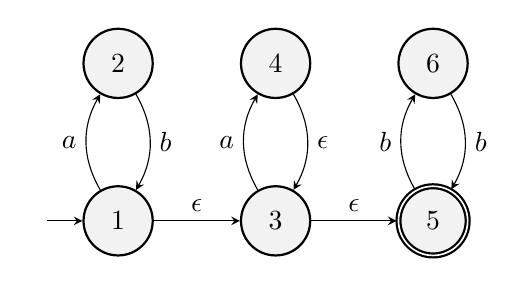
\begin{tikzpicture}
        \node[state,           ] (4) {$4$};
        \node[state, left  of=4] (2) {$2$};
        \node[state, right of=4] (6) {$6$};
        \node[state, initial, below of=2] (1) {$1$};
        \node[state, below of=4] (3) {$3$};
        \node[state, accepting, right of=3] (5) {$5$};
        
        \draw 
        (1) edge[above] node{$\epsilon$} (3)
        (3) edge[above] node{$\epsilon$} (5)
        
        (1) edge[bend left,left] node{$a$} (2)
        (2) edge[bend left,right] node{$b$} (1)
        
        (3) edge[bend left,left] node{$a$} (4)
        (4) edge[bend left,right] node{$\epsilon$} (3)
        
        (5) edge[bend left,left] node{$b$} (6)
        (6) edge[bend left,right] node{$b$} (5);
    \end{tikzpicture}
    \caption{A $\langle 2,3 \rangle$-flat automaton 
that recognizes $L\Def  (ab)^*(a)^*(bb)^*$}
    \label{fig: FA}
\end{figure}

 
\paragraph{Generic Flat Languages and Automata}
Fix $\alpha = \langle p,q \rangle$,
we define the \emph{generic $\alpha$-flat language} is the union of all $\alpha$-flat languages, denoted by $\mathbb{F}(\alpha)$.
Now, we try to define an automaton that recognizes all $\alpha$-flat languages,
i.e., collects all behaviors of $\alpha$-flat automata.

Intuitively, 
the generic automaton is obtained by introducing a new alphabet (
a multi-set with $p q$ copies of the original alphabet) and 
adding more transitions (labels),
the states and the overall framework remain unchanged. 
In details, a generic $\alpha$-flat automaton is still a finite state automaton over
$\Sigma(\alpha)\Def \{a(i)| (a\in \Sigma_\epsilon) \wedge i\in \mathbb{N}:1\le i \le pq\}\cup \{\epsilon\}$.
The states are still named from $1$ to $pq$, 
the initial state is $1$ and the accepting state is $(pq-p+1)$.
The transition relations for state $i$ are defined as 
\begin{itemize}
    \item if $i\  \text{mod}\  p = 1$ and $i\neq pq-p+1$, then 
    $(i,\epsilon,i+p)\in \Delta$
    and $\forall s\in \Sigma_{\epsilon}. (i, s(i) ,i+1) \in \Delta$;
    \item if $i\  \text{mod}\  p = 0$, 
    $\forall s \in \Sigma_{\epsilon}. (i,s(i), i-p+1) \in \Delta$;
    \item otherwise, $\forall s \in \Sigma_{\epsilon}. (i,s(i), i+1) \in \Delta$.
\end{itemize}

For $\Sigma = \{a,b\}$, an example of generic $\langle 2,3 \rangle$-flat automaton is shown in figure (\ref{fig: GFA}).

\begin{figure}[ht]
    \centering 
    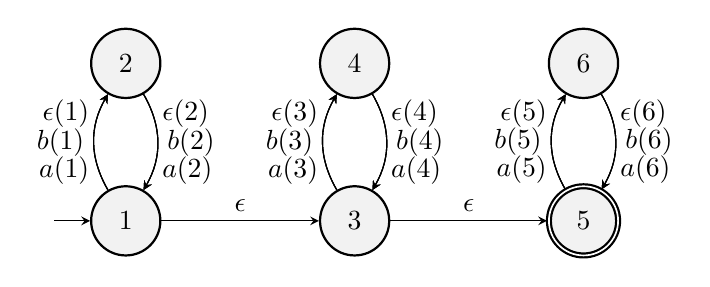
\begin{tikzpicture}
        \node[state,           ] (4) {$4$};
        \node[state, left  = 2cm of 4] (2) {$2$};
        \node[state, right = 2cm of 4] (6) {$6$};
        \node[state, initial, below of=2] (1) {$1$};
        \node[state, below of=4] (3) {$3$};
        \node[state, accepting, below of=6] (5) {$5$};
        
        \draw 
        (1) edge[above] node{$\epsilon$} (3)
        (3) edge[above] node{$\epsilon$} (5)
        
        (1) edge[bend left, pos =0.2 ,left] node{$a(1)$} (2)
        (1) edge[bend left, pos =0.5 ,left] node{$b(1)$} (2)
        (1) edge[bend left, pos =0.8 ,left] node{$\epsilon(1)$} (2)
        
        (2) edge[bend left, pos = 0.2 ,right] node{$\epsilon(2)$} (1)
        (2) edge[bend left, pos = 0.5 ,right] 
        node{$b(2)$} (1)
        (2) edge[bend left, pos = 0.8 ,right] 
        node{$a(2)$} (1)
        
        (3) edge[bend left, pos =0.2 ,left] node{$a(3)$} (4)
        (3) edge[bend left, pos =0.5 ,left] node{$b(3)$} (4)
        (3) edge[bend left, pos =0.8 ,left] node{$\epsilon(3)$} (4)
        
        (4) edge[bend left, pos = 0.2 ,right] node{$\epsilon(4)$} (3)
        (4) edge[bend left, pos = 0.5 ,right] 
        node{$b(4)$} (3)
        (4) edge[bend left, pos = 0.8 ,right] 
        node{$a(4)$} (3)
        
        (5) edge[bend left, pos =0.2 ,left] node{$a(5)$} (6)
        (5) edge[bend left, pos =0.5 ,left] node{$b(5)$} (6)
        (5) edge[bend left, pos =0.8 ,left] node{$\epsilon(5)$} (6)
        
        (6) edge[bend left, pos = 0.2 ,right] node{$\epsilon(6)$} (5)
        (6) edge[bend left, pos = 0.5 ,right] 
        node{$b(6)$} (5)
        (6) edge[bend left, pos = 0.8 ,right] 
        node{$a(6)$} (5);
    \end{tikzpicture}
    \caption{The generic $\langle 2,3 \rangle$-flat automaton}
    \label{fig: GFA}
\end{figure}
 

However,
the resulted automaton may accept languages that are not in $\mathbb{F}(\alpha)$,
because in different passes inside a loop, 
the automaton can choose different symbols between identical pairs. 
To avoid this problem,
we add a so-called purity condition on the accepting language of generic flat automata,
which is equivalent to intersecting the language of a generic flat automaton 
with a language that encodes the purity condition.

We say a string $w\in (\Sigma(\alpha))^*$ is pure if for all $i: 1\le i \le p q$,
and $a,b\in \Sigma$, 
$a\neq b \wedge \#w(a(i))>0$ implies $\#w(b(i))=0$.
Formally, the purity condition is defined by 
\begin{equation} \label{eq:purity}
 \bigwedge_{1\le i\le pq}\bigwedge_{a,b\in \Sigma, a\neq b} ({a(i)}^\#>0)\to ({b(i)}^\#=0)\, . 
\end{equation}

We denote the accepting language of the generic $\alpha$-flat automaton by $\mathbb{G}(\alpha)$.
Note that $\mathbb{G}(\alpha)$ is a language over $\Sigma_\alpha$,
but what we want is a language over $\Sigma$.
So we define a renaming function $R:\Sigma(\alpha)\mapsto \Sigma$ such that for all $a(i) \in \Sigma_\alpha, R(a(i))=a$,
and $R(\epsilon) = \epsilon$.
Define $\mathbb{G}'(\alpha) \, \Def \, \{R(w) \mid w\in \mathbb{G}(\alpha)\}$, 
for simplicity, we write
$\mathbb{G}'(\alpha)=R(\mathbb{G}(\alpha))$.

The important feature of generic flat autamata
is that every word $w\in \mathbb{G}(\alpha)$ is uniquely determined by its Parikh image $\mathbb{P}(w)$.




\section{Flattening string constraints with string-integer conversion}\label{sec:string-solving}

%!TEX root = paper.tex

In this section, we first define the class of string constraints with string-integer conversion, denoted by $\strint$. Then we define the extension of Presburger arithmetic with exponential functions, denoted by $\paexp$. Finally, we show how to flatten the string constraints in $\strint$ into the arithmetic constraints in the existential fragment of $\paexp$. 

\subsection{String constraints with string-integer conversion ($\strint$)}

In the sequel, we shall define $\strint$, the class of string constraints with the string-integer conversion function {\parseInt}.

The function {\parseInt} takes a decimal string as input and returns the integer represented by the string
\footnote{The {\parseInt} function in scripting languages, e.g. Javascript, is more general in the sense that the base can be a number between 2 and 36. Although our approach works for arbitrary positive bases, we choose to focus on the base 10 in this paper, for simplicity.}.
For example, ${\parseInt}($`$0123$'$) = {\parseInt}($`$123$'$)=1*10^2+2*10+3 = 123$. 
Note here we use the quotation marks to delimit strings.

Formally, the semantics of the $\parseInt$ function is defined as follows. 
In order to simplify the presentation, we assume all string variables ranging over numerical symbols $\Sigma_{\textit{num}}=\{0,1, \ldots, 9\}$. 
Note that one can easily extend our approach to allow arbitrary finite alphabet. Then ${\parseInt}: \Sigma_{\textit{num}}^+ \mapsto \Nat$ is recursively defined by, for every $w\in \Sigma_{\textit{num}}^+$,
\begin{itemize}
    \item if $w=$`$i$' for $i \in \Sigma_{\textit{num}}$, then ${\parseInt}$$($`$i$'$)=i$;
    \item for $w = w'\cdot$`$i$' for $i \in \Sigma_{\textit{num}}$ with $\len(w') \ge 1$, 
        ${\parseInt}(w) = 10*{\parseInt}(w')+{\parseInt}($`$i$'$)$.
\end{itemize} 
Note that $\parseInt$ is undefined with $\varepsilon$ as the input.

%%%%%%%%%%%%%%%%%%%%%%%%%%%%%%%
\hide{
In $\strint$, there are two types of variables, i.e. the string variables $\svarx,\svary,\ldots \in \svars$ and the integer variables $\ivarx,\ivary,\ldots \in \ivars$.
A $\strint$ formula $\varphi$ is defined by the following rules, where $\len(\sterm)$ denotes the length of a string $\sterm$.
\[
\begin{array}{l c l}
\sterm & \Def & a \mid \svarx \mid \sterm \cdot \sterm, \\
\iterm & \Def & n \mid \ivarx \mid \len(\sterm) \mid \parseInt(\sterm) \mid \iterm + \iterm \mid \iterm - \iterm,\\
\varphi & \Def & \sterm = \sterm \mid x \in \Aut \mid \iterm\ \op\ \iterm \mid \varphi \wedge \varphi \mid \varphi \vee \varphi \mid \neg \varphi,
\end{array}
\]
where $a \in (\Sigma_{\textit{num}})_\varepsilon$, $n \in \Nat$, $\Aut$ is an FA, and $\op \in \{=, < , >, \le, \ge\}$. Let us call $\sterm$ as string terms, $\iterm$ as integer terms, $\sterm = \sterm$ as string equality constraints, $x \in \Aut$ as regular constraints, $\iterm \op\ \iterm$ as arithmetic constraints. 
Let  $\svar(\varphi)$ and $\ivar(\varphi)$ denote the set of string variables and integer variables respectively occurring in $\varphi$.
}
%%%%%%%%%%%%%%%%%%%%%%%%%%%%%%%%%%%


In $\strint$, there are two types of variables, i.e. the string variables $\svarx,\svary,\ldots \in \svars$ and the integer variables $\ivarx,\ivary,\ldots \in \ivars$.
The syntax of $\strint$ is defined as follows:
a string term, denoted by $\sterm$, is of the form 
$$\sterm\  \Def\  a \mid \svarx \mid \sterm \cdot \sterm,$$
an integer term, denoted by $\iterm$, is of the form
$$\iterm\  \Def\  c \mid \ivarx \mid \len(\sterm) \mid \parseInt(\sterm) \mid \iterm + \iterm \mid \iterm - \iterm,$$
and a $\strint$ formula, denoted by $\varphi$ is of the form 
$$\varphi\ \Def\ \sterm = \sterm \mid \sterm \in \Aut \mid \iterm\ \op\ \iterm \mid \varphi \wedge \varphi \mid \varphi \vee \varphi \mid \neg \varphi$$
where $a \in (\Sigma_{\textit{num}})_\varepsilon$, $c \in \mathbb Z$, $\Aut$ is an FA, $\op \in \{=, < , >, \le, \ge\}$ and $\len(\sterm)$ denotes the length of a string $\sterm$. 
Let us call $\sterm = \sterm$ as string equality constraints, $\sterm \in \Aut$ as regular constraints, $\iterm \op \iterm$ as arithmetic constraints. 
Let  $\svar(\varphi)$ and $\ivar(\varphi)$ denote the set of string variables and integer variables occurring in $\varphi$ respectively.

The $\strint$ formulas are interpreted on $I=(I_s, I_i)$ where $I_s$ is a partial function from $\svars$ (the set of string variables) to $\Sigma^*$ and $I_i$ is a partial function from $\ivars$ (the set of integer variables) to $\mathbb Z$. 
% nat -> Z
Moreover, it is required that the domains of $I_s, I_i$ are finite. Given $I = (I_s, I_i)$, the interpretations of string terms, integer terms, as well as the formulas $\varphi$ under $I$ are easy to comprehend, thus omitted to avoid tediousness. 
For $\varphi \in \strint$ and $I = (I_s, I_i)$, $I$ satisfies $\varphi$ if the interpretation of $\varphi$ under $I$ is $\ltrue$.
Let us use $\lVert \varphi \rVert$ to denote the set of $I = (I_s, I_i)$ satisfying $\varphi$.

\begin{example} Given a FA $\Aut$, the constraint
$$\svarx \in \Aut \ \wedge\ 
\parseInt(\svarx) = 109\ivarx\ \wedge\ 
\len(\svarx) < 100$$
is a $\strint$ formula.
\end{example}

The satisfiability problem of $\strint$ is to decide for a given constraint $\varphi \in \strint$,
whether $\lVert  \varphi \rVert \neq \emptyset$.

\subsection{Presburger Arithmetic with Exponential Functions (\paexp)}

{\paexp} extends Presburger arithmetic with two partial functions, the \emph{exponential} function $10^\ivarx$ and the \emph{integer logarithmic} function $\ell_{10}(\ivarx)$ (cf. \cite{Point86}). The function $\ell_{10}(\ivarx)$ is defined as follows: for $n \ge 1$, $\ell_{10}(n) = m$ if $10^m \le n < 10^{m+1}$. Note that $10^\ivarx$ is undefined for $\ivarx<0$ and $\ell_{10}(\ivarx)$ is undefined for $\ivarx\le 0$.

The syntax of {\paexp} is obtained from that of {\pa} by adding $10^\iterm$ and $\ell_{10}(\iterm)$ to the definition of terms. An {\paexp} term, denoted by $\iterm$, is of the form
$$\iterm\ \Def\ c \mid \ivarx \mid \iterm + \iterm \mid \iterm - \iterm \mid 10^{\iterm} \mid \ell_{10}(\iterm) $$
where $\ivarx$ is an integer variable and $c\in \mathbb Z$ is an constant integer. In addition, we require that $10^\iterm$ and $\ell_{10}(\iterm)$ terms are well-defined, which restricts the interpretations of $\iterm$ therein.

A formula of {\paexp}, denoted by $\phi$, is of the form
$$\phi \ \Def \ \iterm \ \op\ \iterm \mid c \vert \iterm \mid c \nmid \iterm \mid \neg \phi \mid \phi \wedge \phi \mid \phi \vee \phi \mid \exists \ivarx.\ \phi \mid \forall \ivarx.\ \phi,$$
where $\op \in \{=, < , >, \le, \ge\}$. 

The semantics of {\paexp} are defined similarly to that of {\pa} with the only difference that partial functions are required to be well-defined. The quantifier-free and existential {\paexp} formulas are defined similarly to {\pa} as well.
We also assume that quantifier-free {\paexp} formulas are free of negations, for the same reason we have explained for {\pa}.

\hide{
The semantics of {\paexp} are defined similarly to {\pa} with the only difference that variables are interpreted over $\Nat$ rather than $\mathbb Z$, that is, an interpretation is a function $I:\free(\phi)\to \mathbb \Nat$. 
This restriction ensures that terms $10^\iterm$ and $\ell_{10}(\iterm)$ are well-defined: In the \emph{normalization} step of the quantifier elimination procedure, for each $\ell_{10}(\iterm)$ term, we will replace all its occurrences by a fresh variable $\ivarz$, and add a conjunct $10^\ivarz \le \iterm < 10\cdot 10^\ivarz$. 
Then $\ivarz\in\Nat$ guarantees that $\iterm \ge 1$ is always satisfied.
Exponential functions are treated similarly
(more details can be found in Section~\ref{qe-norm}).
Note that we can extend the interpretation to $\mathbb Z$ since each integer can be written as the difference of two positive integers.
}

For convenience, when working with exponential and logarithmic functions, we use the notation $\lambda_{10}(\iterm)$ to denote $10^{\ell_{10}(\iterm)}$. It is easy to show that for all $n \ge 1$, $\lambda_{10}(n) \le n < 10\lambda_{10}(n)$ holds.

\begin{example}
$10^{10^\ivarx}+10^{\ivarx+ \ivary} + 3\ivary    = 2 \ivarz +1 $ is an {\paexp} formula.
\end{example} 
 
\subsection{Flattening $\strint$ into $\paexp$}

We first recall the flattening approach for string constraints in \cite{Parosh:20:PLDI}, then show how to extend it to deal with {\parseInt}.

A \emph{flat domain restriction} for a string constraint $\varphi\in \strint$ is a function $\flatfun_\varphi$ that maps each string variable $\svarx \in \svar(\varphi)$ to a flat language $(w_{\svarx,1})^* \cdots (w_{\svarx, k_\svarx})^*$, where $w_{\svarx, i} \in \Sigma_{\textit{num}}^+$ for every $i \in [k_\svarx]$. 
The flattened semantics of $\varphi \in \strint$ is defined as $\llbracket \varphi \rrbracket_{\flatfun_\varphi} = \{(I_s, I_i) \in \llbracket \varphi  \rrbracket \mid \forall \svarx \in \svar(\varphi).\ I_s(x) \in  \flatfun_\varphi(\svarx)\}$.  

%%%%%%%%%%%%%%%%%%%%%%%%%%%%%%%%%%%%%%%%%%
\hide{
The flattening of $\varphi \in \strint$ under a flat domain restriction $\flatfun_\varphi$ is a {\paexp} formula, denoted by $\flatten_{\flatfun_\varphi}(\varphi)$, that encodes its flattened semantics.
More concretely, $\flatten_{\flatfun_\varphi}(\varphi)$ is a formula over the integer variables $\ivar(\varphi)$,  and flattening variables $\pvar_{\flatfun_\varphi}(\varphi) = \bigcup_{\svarx \in \svar(\varphi)} \pvar_{\flatfun_\varphi}(\svarx)$, where $\pvar_{\flatfun_\varphi}(\svarx) = \{l_{\svarx,i} \mid i \in [k_\svarx]\}$, plus some other auxiliary variables, such that 
$$\llbracket \varphi \rrbracket_{\flatfun_\varphi} =\decode_{\flatfun_\varphi}(\llbracket \flatten_{\flatfun_\varphi}(\varphi) \rrbracket \vert_{\ivar(\phi) \cup \pvar_{\flatfun_\varphi}(\varphi)}).$$
}
%%%%%%%%%%%%%%%%%%%%%%%%%%%%%%%%%%%%%%%%%

Under a flat domain restriction $\flatfun_\varphi$, the flattening of $\varphi \in \strint$ is an $\paexp$ formula, denoted by $\flatten_{\flatfun_\varphi}(\varphi)$, that encodes the flattened semantics $\llbracket \varphi \rrbracket_{\flatfun_\varphi}$. 
The idea is that $x$ can be expressed as $(w_{\svarx,1})^{l_{x,1}} \cdots (w_{\svarx, k_\svarx})^{l_{x,k_x}}$ with $l_{x,i}$ denoting the number of iterations of $w_{x,i}$,  
so we can eliminate the occurrences of $x$ in $\varphi$ by introduce a set of integer variables $\pvar_{\flatfun_\varphi}(\svarx) = \{l_{\svarx,i} \mid i \in [k_\svarx]\}$. 
More concretely, $\flatten_{\flatfun_\varphi}(\varphi)$ is a formula over the integer variables $\ivar(\varphi)$,  and flattening variables $\pvar_{\flatfun_\varphi}(\varphi) = \bigcup_{\svarx \in \svar(\varphi)} \pvar_{\flatfun_\varphi}(\svarx)$ plus some other auxiliary variables, such that the interpretations $I_e: \ivar(\varphi) \cup \pvar_{\flatfun_\varphi}(\varphi) \rightarrow \mathbb Z$ of $\llbracket \flatten_{\flatfun_\varphi}(\varphi) \rrbracket$and interpretations $(I_s, I_i)$ of $\llbracket \varphi \rrbracket_{\flatfun_\varphi}$ have the following correspondence 

\begin{itemize}
    \item  
    for every $ \svarx \in \svar(\varphi)$, $I_s(\svarx) = w_{\svarx,1}^{I_e(l_{\svarx,1})} \ldots  w_{\svarx,k_\svarx}^{I_e(l_{\svarx,k_\svarx})}$, where $I_e(l_{x,i})\ge 0$ for $1\le i\le k_x$.
    %
    \item for every $ \ivarx \in \ivar(\varphi)$, $I_i(\ivarx) = I_e(\ivarx)$.
\end{itemize}

%%%%%%%%%%%%%%%%%%%%%%%%%%%%%%
\hide{
$$\llbracket \varphi \rrbracket_{\flatfun_\varphi} =\decode_{\flatfun_\varphi}(\llbracket \flatten_{\flatfun_\varphi}(\varphi) \rrbracket \vert_{\ivar(\phi) \cup \pvar_{\flatfun_\varphi}(\varphi)}).$$

The decoding function above decodes an interpretation of integer and flattening variables $I_e: \ivar(\varphi) \cup \pvar_{\flatfun_\varphi}(\varphi) \rightarrow \mathbb Z$ as a set $\decode_{\flatfun_\varphi}(I_e)$ of interpretations of the $\varphi$'s integer and string variables $(I_s, I_i)$ with $I_s: \svar(\varphi) \rightarrow \Sigma^*$ and $I_i: \ivar(\phi) \rightarrow \Nat$ such that 
}
%%%%%%%%%%%%%%%%%%%%%%%%%%%%%%

The formula $\flatten_{\flatfun_\varphi}(\varphi)$ is constructed inductively on the structure of $\varphi$: $\flatten_{\flatfun_\varphi}(\varphi_1\ \mathfrak{o}\ \varphi_2) = \flatten_{\flatfun_\varphi}(\varphi_1) \ \mathfrak{o}\  \flatten_{\flatfun_\varphi}(\varphi_2)$, where $\mathfrak{o} \in \{\wedge, \vee\}$, and $\flatten_{\flatfun_\varphi}(\neg \varphi_1) = \neg \flatten_{\flatfun_\varphi}(\varphi_1)$. Therefore, it is sufficient to show how to construct $\flatten_{\flatfun_\varphi}(\varphi)$ for atomic constraints $\varphi$. 
In the sequel, we will show how to construct $\flatten_{\flatfun_\varphi}(\iterm_1 \op \iterm_2)$ where $\parseInt(\sterm)$ may occur in $\iterm_1$ or $\iterm_2$. The construction of $\flatten_{\flatfun_\varphi}(\varphi)$ for the other atomic constraints is omitted because it is essentially the same as that in \cite{Parosh:20:PLDI} (we summarize as Theorem~\ref{thm:string}).

\begin{theorem}\label{thm:string}\cite{Parosh:20:PLDI} The satisfiability of Boolean combinations of string equality constraints, regular constraints and arithmetic constraints under flat domain restrictions can be reduced to the satisfiability of existential {\pa}   formulas, thus is decidable.
\end{theorem}

For simplicity, we assume that each occurrence of $\parseInt$ (resp. $\len(t)$) in $\iterm_1 \op \iterm_2$ is of the form $\parseInt(\svarx)$ (resp. $\len(\svarx)$) for a string variable $\svarx$. (Otherwise, we can introduce a fresh variable $\svarx'$ for $\sterm$ in $\parseInt(\sterm)$ or $\len(\sterm)$ and add the constraint $\svarx' = \sterm$.)
Then $\flatten_{\flatfun_\varphi}(\iterm_1 \op \iterm_2)$ is obtained from $\iterm_1 \op \iterm_2$ by replacing $\parseInt(\svarx)$ with $\flatten_{\flatfun_\varphi}(\parseInt(\svarx))$ and $\len(\svarx)$ with $\flatten_{\flatfun_\varphi}(\len(\svarx))$, where 
\begin{itemize}
\item 
$\flatten_{\flatfun_\varphi}(\parseInt(\svarx)) \Def \iterm_{\svarx,1}$  such that $(\iterm_{\svarx, i})_{i \in [k_\svarx]}$ are inductively defined as follows: 
\begin{itemize}
\item for $i = k_\svarx$, 
$$\iterm_{\svarx, i} = \frac{\parseInt(w_{\svarx, k_\svarx}) (10^{\len(w_{\svarx,k_\svarx})l_{\svarx, k_\svarx}} -1 )}{(10^{\len(w_{\svarx, k_\svarx}) } -1 )}$$ 
%
\item for $i \in [k_\svarx-1]$, 
%
$$ \hspace{-1.2cm} \iterm_{\svarx, i} =  \frac{\parseInt(w_{\svarx, i}) (10^{\len(w_{\svarx, i})  l_{\svarx, i} } -1 ) 10^{\big(\sum_{i+1\le j\le k_x} \len(w_{\svarx, j})  l_{\svarx, j}\big)}} {(10^{\len(w_{\svarx, i}) } -1 )} + \iterm_{\svarx, i+1}$$
\end{itemize}
%
\item Notice that here $\len( w_{\svarx, \textunderscore } )$ are constants while $l_{\svarx, \textunderscore}$ are (flattening) variables. So we have 
$$\flatten_{\flatfun_\varphi}(\len(\svarx)) \Def \sum \limits_{i \in [k_{\svarx}]} \len(w_{\svarx, i})  l_{\svarx, i}.$$ 
\end{itemize} 

The following example helps to illustrate the main idea of the flattening technique.

\begin{example}
Suppose $\parseInt(\svarx) = 2\ivarx$ is an atomic constraint and $\flatfun_\varphi(\svarx) = 1^*2^*$. Then 
\[
\small
\begin{array}{l l}
& \flatten_{\flatfun_\varphi}(\parseInt(\svarx)  =  2\ivarx)  \\
\Def & 1 \frac{10^{l_{\svarx,1}}-1}{10-1}10^{l_{\svarx,2}}  + 2 \frac{10^{l_{\svarx,2}}-1}{10-1} = 2\ivarx   \\
\equiv & 10^{l_{\svarx,1}+l_{\svarx,2}} - 10^{l_{\svarx,2}}  + 2*10^{2l_{\svarx,2}}- 2 = 18\ivarx \\
\equiv & 10^{l_{\svarx,1}+l_{\svarx,2}} +  10^{l_{\svarx,2}} = 18\ivarx + 2.
\end{array}
\]
\end{example}

By Theorem~\ref{thm:string}, the above reduction, and the decidability of $\paexp$'s satisfiability (see Theorem~\ref{thm-paexp}), we have 
\begin{theorem} \label{thm:string-parInt}
    The satisfiability of  $\strint$ under flat domain restrictions can be reduced to the satisfiability of existential $\paexp$ formulas, and thus is decidable.
\end{theorem}


\section{Decision procedure for $\paexp$}

%!TEX root = paper.tex

Sem\"{e}nov first proved that  {\paexp} admits quantifier elimination in \cite{Semenov84}, thus its satisfiability problem is decidable. However, Sem\"{e}nov did not give a concrete quantifier elimination algorithm. Remedying this, Point proposed a quantifier elimination algorithm for {\paexp} in \cite{Point86}. 
The goal of this section is to illustrate how Point's quantifier elimination algorithm works. Moreover, we give a complexity analysis to Point's algorithm, which was missing in \cite{Point86}.
%
\begin{theorem}\label{thm-paexp}
{\paexp} admits quantifier elimination of doubly-exponential complexity.
\end{theorem}
%
As Point's algorithm is quite expensive and a faithful implementation would not scale\footnote{We did implemented Point's algorithm and discovered that the implementation could only solve formulas of very small size.}, in the next section, we will propose various optimizations to Point's algorithm, aiming at an efficient implementation. 

In the sequel, we are going to show that every {\paexp} formula $\exists \ivarx.\ \varphi \in \paexp$, where $\varphi$ is quantifier-free, can be transformed into an equivalent quantifier-free formula $\varphi' \in \paexp$.
% such that $\free(\varphi') = \free(\varphi) \setminus \{\ivarx\}$. 
%From this, we can easily derive that every {\paexp} formula $\varphi$ can be transformed effectively into an equivalent quantifier-free Presburger arithmetic formula $\varphi'$.

Before a formal description of the quantifier elimination procedure, let us use a simple example to illustrate the main idea and give an overview of the procedure.

%\begin{example}
\subsection{An overview of the quantifier elimination procedure}
Consider $\varphi \Def \exists \ivarx_2.\ 10^{\ivarx_1 + \ivarx_2} - 10^{\ivarx_2} \le \ivary + 1001$. 

At first, we \emph{normalize} $\varphi$ by introducing a fresh variable $\ivarx_3$ for $\ivarx_1 + \ivarx_2$ and get the formula 
$$\varphi_1 \Def \exists \ivarx_3 \exists \ivarx_2.\ 10^{\ivarx_3} - 10^{\ivarx_2} \le \ivary + 1001 \wedge \ivarx_3 = \ivarx_1 + \ivarx_2.$$

Then, we enumerate different \emph{orders} of the quantified variables, i.e. $\ivarx_2$ and $\ivarx_3$. Since $\ivarx_3 = \ivarx_1 + \ivarx_2$, there is only one possible order, that is, $\ivarx_3 \ge \ivarx_2$.

Next, we illustrate how to eliminate the quantifier $\exists \ivarx_3$, assuming $\ivarx_3 \ge \ivarx_2$. The elimination of $\exists \ivarx_2$ is similar and simpler, thus omitted.

The elimination of $\exists \ivarx_3$ consists of two steps, namely, eliminating the exponential occurrences of $\ivarx_3$ first, and the linear occurrences next.

The main idea of the elimination of the exponential occurrences of $\ivarx_3$ is to observe that if $\ivarx_3 \ge \ell_{10}(\ivary+1001)+2$ and $\ivarx_3 \ge \ivarx_2 + 3$, then $10^{\ivarx_3} - 10^{\ivarx_2}$ is dominated by $10^{\ivarx_3}$, that is, $10^{\ivarx_3} - 10^{\ivarx_2} \ge 10^{\ivarx_3} - 10^{\ivarx_3 - 3} = (1-10^{-3}) 10^{\ivarx_3} \ge 10^{\ell_{10}(\ivary+1001)+1} = 10\lambda_{10}(\ivary+1001) > \ivary+1001$. Therefore, a necessary condition for $10^{\ivarx_3} - 10^{\ivarx_2} \le \ivary + 1001$ is that either $\ivarx_3 \le \ell_{10}(\ivary+1001)+1$ or $\ivarx_3 \le \ivarx_2 + 2$ holds.  
\begin{itemize}
\item If $\ivarx_3 \le \ell_{10}(\ivary+1001)+1$, then we distinguish between whether $\ivarx_3 \le \ell_{10}(\ivary+1001)$ or  $\ivarx_3 = \ell_{10}(\ivary+1001)+1$. 
\begin{itemize}
\item If $\ivarx_3 \le \ell_{10}(\ivary+1001)$, then $10^{\ivarx_3} - 10^{\ivarx_2} \le 10^{\ell_{10}(\ivary+1001)} = \lambda_{10}(\ivary+1001) \le \ivary + 1001$. In this case, $10^{\ivarx_3} - 10^{\ivarx_2} \le \ivary + 1001 \wedge \ivarx_3 = \ivarx_1 + \ivarx_2$ can simplified into $\ltrue$.
%
\item If $\ivarx_3 = \ell_{10}(\ivary+1001)+1$, then $10^{\ivarx_3} - 10^{\ivarx_2} \le \ivary + 1001$ can be turned into $10^{\ell_{10}(\ivary+1001)+1} - 10^{\ivarx_2} \le \ivary + 1001 \equiv 10 \lambda_{10}(\ivary+1001) - 10^{\ivarx_2} \le \ivary + 1001 $.
\end{itemize} 
%
\item If $\ivarx_3 \le \ivarx_2 + 2$, then $\ivarx_3 = \ivarx_2 + j$ for $j \in \{0,1,2\}$. Thus $10^{\ivarx_3} - 10^{\ivarx_2} \le \ivary + 1001$ can be transformed to $\bigvee \limits_{j \in \{0,1,2\}} 10^{\ivarx_2 + j} - 10^{\ivarx_2} \le \ivary + 1001$.
\end{itemize}

To summarize, $\varphi_1$ is transformed into 
\[
\small
\begin{array}{l}
\varphi_2 \Def \exists \ivarx_3 \exists \ivarx_2. \\
\begin{array}{l}
\vspace{2mm}
\left(
\begin{array}{l}
\ivarx_3 \le \ell_{10}(\ivary+1001)\ \vee \\
\left(
\begin{array}{l}
\ivarx_3 = \ell_{10}(\ivary+1001)+1\ \wedge \\
10 \lambda_{10}(\ivary+1001) - 10^{\ivarx_2} \le \ivary + 1001 
\end{array}
\right) \vee \\
%
 \bigvee \limits_{j \in \{0,1,2\}}  \left(\ivarx_3 = \ivarx_2 +j \wedge 10^{\ivarx_2 + j} - 10^{\ivarx_2} \le \ivary + 1001\right)
\end{array}
\right) 
\wedge \\
 \ivarx_3 = \ivarx_1 + \ivarx_2.
 \end{array}
\end{array}
\]
Note that $\varphi_2$ contains \emph{only linear} occurrences of $\ivarx_3$.

Finally, we can eliminate the linear occurrences of $\ivarx_3$, thus the quantifier $\exists \ivarx_3$, by applying the quantifier elimination algorithm of {\pa}, e.g. Cooper's algorithm in \cite{Cooper72}. The elimination of $\ivarx_3$ in $\varphi_2$ is simple, with $\ivarx_3$ replaced by $\ivarx_1 + \ivarx_2$, resulting into  
\[
\small
\begin{array}{l}
\varphi_3 \Def \exists \ivarx_2.\ 
\ivarx_1 + \ivarx_2 \le \ell_{10}(\ivary+1001)\ \vee \\
\left(
\begin{array}{l}
\ivarx_1 + \ivarx_2 = \ell_{10}(\ivary+1001)+1\ \wedge \\
10 \lambda_{10}(\ivary+1001) - 10^{\ivarx_2} \le \ivary + 1001 
\end{array}
\right) \vee \\
%
 \bigvee \limits_{j \in \{0,1,2\}}  \left(\ivarx_1 + \ivarx_2 = \ivarx_2 +j \wedge 10^{\ivarx_2 + j} - 10^{\ivarx_2} \le \ivary + 1001\right).
\end{array}
\]

\smallskip

In the remainder of this section, we are going to describe the aforementioned steps of the decision procedures: Normalization, the enumeration of the variable orders, 
the elimination of the exponential occurrences of variables. The elimination of the  linear occurrences of variables is essentially the quantifier elimination of the {\pa} and omitted.

Let us assume that $\varphi \Def \exists \ivarx.\ \varphi'(\ivarx, \vec{\ivary})$, where $\varphi'$ is a quantifier-free formula. 


%%%%%%%%%%%%%%%%%%%%%%%%%%%%%%%%%%%%%%%%%%%%%%
%%%%%%%%%%%%%%%%%%%%%%%%%%%%%%%%%%%%%%%%%%%%%%
\hide{
\begin{definition}
    For a strictly increasing function $f:\mathbb{N}\mapsto \mathbb{N}$, 
    $f$ is said to be \emph{compatible with addition}
    if for every $m\in \mathbb{N}^+$,  $f$ modulo $m$ is periodic, 
    and for any term $A(x)=\sum_{1\le i\le n} a_i f(x+b_i)$, 
    where $n \in \mathbb{N}^+, a_i ,b_i \in \mathbb{Z}$,
    one of the following holds:
    \begin{itemize}
        \item $A(x)$ is bounded; 
        \item there exists a constant $\Delta_A\in \mathbb{N}^+$ such that 
        $\forall x. A(x+\Delta_A)\ge f(x)$;
        \item there exists a constant $\Delta_A\in \mathbb{N}^+$ such that 
        $\forall x. -A(x+\Delta_A)\ge f(x)$.
    \end{itemize}
\end{definition}

Semenov proved that for any function $f$ that is compatible with addition, the first order theory $(\mathbb{N},+,f)$ admits QE  and thus is complete and decidable \cite{Semenov84}. Exponential functions are a typical class of compatible with addition functions, and therefore {$\paexp$} is decidable. Particularly, in \cite{Point86} 
Point gave a detailed QE algorithm for $(\mathbb{N},+,2^x)$.
%下面这些感觉可以不用说,或者放在后面
%Unfortunately, Point's algorithm is flawed, one problem lies in the discussion to eliminate exponential terms. For example, after  eliminating variable $x$ in formula $\exists x. y\le 2^x \wedge x\le 10$, the expected result should be $y\le 2^{10} =1024$, but Point's algorithm will return a formula equivalent to $y \le 2^6=64$.

In this section, within Point's framework, we give a revised algorithm to the decision problem of {$\paexp$} with both improvements and corrections, that provides a crucial step to the decision procedure of string constraints with {\parseInt} function according to Theorem~\ref{thm:string-parInt}. 

%\section{Quantifier Elimination Algorithm for $(\mathbb{N},+,2^x)$}
% Based on Point's work \cite{Point86}, 
We will present a revised QE algorithm for {$\paexp$} formulas of the form $Qx.\theta(x,\bar{y})$, where $Q$ is a quantifier and $\theta(x,\bar{y})$ is a quantifier-free formula. Since $\forall x. F = \neg \exists x. \neg F$, we further assume the quantifier is an existential quantifier, that is, $\exists x.\theta(x,\bar{y})$. For eliminating quantifiers in arbitrary {$\paexp$} formula, we need to apply the algorithm to the innermost quantified formula and repeat this procedure until all quantifiers are eliminated.

The whole QE algorithm can be divided into 4 steps. The first step \textbf{Normalization} can be viewed as a pre-processing step, which substitutes ``complex" terms like $2^{2^x}$, $l_2(3x+y)$ with ``simple" terms by introducing new variables. After \textbf{Normalization}, we move forward to handle a ``simpler" formula, however, at the cost of more quantified variables.

The other three steps undertake the task to eliminate the newly introduced variables in \textbf{Normalization} step, denoted by $\{x_i:1\le i\le n\}$, and the original variable $x$ (will be denoted by $x_0$) one by one. 
The main body of \textbf{Enumerate-Orders} step is a loop to enumerate all possible orders among quantified variables $\{x_i : 0\le i \le n\}$. 
In each iteration, according the given (decreasing) order of quantified variables (corresponding to an outer \emph{for} loop), we invoke \textbf{Elim-exp} and \textbf{Elim-linear} to eliminate these variables one by one. 

During each iteration of the inner \emph{for} loop, if the maximal $x_i$ in $\bar{x}$ occurs in an exponential term in an atom, we will invoke \textbf{Elim-exp} to produce an equivalent formula where $x_i$ occurs linearly. Then \textbf{Elim-linear} will eliminate all linear occurrences of $x_i$, which is similar to the classic Cooper's QE algorithm for PA \cite{Cooper72}. 

A more detailed description is given below.
}
%%%%%%%%%%%%%%%%%%%%%%%%%%%%%%%%%%%%%%%%%%%%%%
%%%%%%%%%%%%%%%%%%%%%%%%%%%%%%%%%%%%%%%%%%%%%%


\subsection{Normalization}

%%%%%%%%%%%%%%%%%%%%%%%%%%%%%%%%%
%%%%%%%%%%%%%%%%%%%%%%%%%%%%%%%%%
\hide{
In order to show $(\mathbb{N},+,2^x)$ admits QE , 
it is sufficient to show that any 1-existential formula $\exists x.\theta(x,\bar{y})$ indeed does, 
where $\theta(x,\bar{y})$ is a quantifier-free formula. 
However, the form of $\exists x.\theta(x,\bar{y})$ is unknown so it may contain terms difficult to handle such as $2^{3x+y+1}$ or $l_2(x)$.
The \textbf{Normalization} step simplifies these terms by introducing new variables, 
for example, $\exists x.2^{3x+y+1}>10$ is equivalent to
$$\exists x\exists x_1.2^{x_1}>10 \wedge x_1 =3x+y+1\,.$$

Logarithm functions are replaced by exponential functions, take $\exists x.l_2(x)>3$ for example, $l_2(x)$ is replaced by a new variable $x_1$, and we have  
$$\exists x\exists x_1. x_1 > 3 \wedge 2^{x_1}\le x \wedge x\le 2^{x_1+1}-1\,.$$
}
%%%%%%%%%%%%%%%%%%%%%%%%%%%%%%%%%
%%%%%%%%%%%%%%%%%%%%%%%%%%%%%%%%%

The normalization step comprises the following sub-steps.
\begin{enumerate}
\item At first, we transform $\varphi'(\ivarx,\vec{\ivary})$ into the NNF (negation normal form). Moreover, we remove the occurrences of $\neg$ by replacing $\neg c | \iterm$ with $\bigvee \limits_{j \in [c-1]} c | (\iterm+j)$, $\neg \iterm_1 = \iterm_2$ with $\iterm_1 < \iterm_2 \vee \iterm_2 < \iterm_1$, $\neg \iterm_1 < \iterm_2$ with $\iterm_2 \le \iterm_1$, $\neg \iterm_1 \le \iterm_2$ with $\iterm_2 < \iterm_1$, and so on.
%
\item Repeat the following procedure, until there are no $\lambda_{10}(\iterm)$ where $\ivarx$ occurs: Replace each occurrence of $\lambda_{10}$ in $\varphi'$, say $\lambda_{10}(\iterm)$, such that $\ivarx$ occurs in $\iterm$, by $10^{\ell_{10}(\iterm)}$. Let the resulting formula be $\varphi''$.
%
\item Then repeat the following procedure to $\varphi''$, until for each occurrence of $10^{\iterm}$ where $\ivarx$ occurs, we have $\iterm = \ivarx$: For each occurrence of the $\ell_{10}$ in $\varphi''$, say $\ell_{10}(\iterm)$, such that it contains $\ivarx$ but is not $\ivarx$, introduce a fresh variable, say $\ivarz$, 
%and let $\varphi''':= \exists \ivarz.\ \varphi''[\ivarz/\ell_{10}(\iterm)] \wedge 10^\ivarz \le \iterm < 10^{\ivarz + 1}$. 
and replace all occurrences of $\ell_{10}(\iterm)$ by $\ivarz$, moreover, add the constraint $10^\ivarz \le \iterm < 10^{\ivarz + 1}$ as a conjunct. Let $\varphi'''$ denote the resulting formula.  
%
\item Do the following replacements to $\varphi'''$ so that all the atomic formulas are of the form $\iterm_1 \le \iterm_2$ or $c | \iterm$: Replace every occurrence of $\iterm_1 \ge \iterm_2$ with $\iterm_2 \le \iterm_1$. Replace every occurrence of $\iterm_1 < \iterm_2$ (resp. $\iterm_1 > \iterm_2$) with $\iterm_1 \le \iterm_2 - 1$ (resp. $\iterm_2 \le \iterm_1-1$). Replace ever occurrence of $\iterm_1 = \iterm_2$ wtih $\iterm_2 \le \iterm_1 \wedge \iterm_1 \le \iterm_2$. Let $\varphi^\dag$ the resulting formula. 
%
\item Let $\vec{\ivarz} = \ivarz_1,\ldots, \ivarz_n$ be an enumeration of the freshly introduced variables. Then the result of the normalization procedure is 
$\exists \vec{\ivarz}\exists \ivarx.\ \varphi^\dag$.
\end{enumerate}


%%%%%%%%%%%%%%%%%%%%%%%%%%%%%%%%%%%%%%%%%%%%%%%
%%%%%%%%%%%%%%%%%%%%%%%%%%%%%%%%%%%%%%%%%%%%%%%
\hide{
Then $\theta(x,\bar{y})$ becomes a Boolean combination (with only $\wedge$ and $\vee$) of literals.

Make substitutions by introducing new variables according to the \textit{while} statements in the pseudo-code. For consistency, we rename the original $x$ to be $x_0$ and assume $n$ new quantified variables are introduced.

%After introducing new variables and substitution, 
After substitutions, we obtain a formula where if an exponential term contains a quantified variable $x_i$, the term must be $2^{x_i}$.
We then collect all terms with $x_i (0\le i\le n)$ together, it will be of the form $s(\bar{x}) \Def \sum_{i=0}^{n} a_i 2^{x_i} + \sum_{i=0}^n b_i x_i$, where $a_i,b_i (0\le i \le n)$ are all constants.
Other terms including constants and terms of free variables $\bar{y}$ are collected, denoted by $t(\bar{y})$. Since $\bar{y}$ are free variables, we will regard $t(\bar{y})$ as a constant. Inequalities and equalities will all be transformed into $s(\bar{x})\le t(\bar{y})$, for example, $s(\bar{x}) = t(\bar{y})$ will be replaced by $s(\bar{x})\le t(\bar{y})\wedge t(\bar{y})\le s(\bar{x})$.
 end, the resulted formula $\theta'$ only contains literals of the forms $s(\bar{x})\le t(\bar{y})$, $k|s(\bar{x})+t(\bar{y})$ and $\neg  (k|s(\bar{x})+t(\bar{y}))$.


\begin{algorithm}[t]
    \SetAlgoLined
    \KwIn{1-existential formula $\exists x.\theta(x,\bar{y})$}
    \KwOut{n-existential formula $\exists \bar{x}.\theta'(\bar{x},\bar{y})$}
    
    $\theta' :=  \theta(x,\bar{y})$ \;
    Transform $\theta'$ into NNF\;
    \tcp{ i is used for counting the introduced variables }
    $i := 1$\; 
    \tcp{ $\bar{y}$ are regarded as constants} 
    \While{there is a term $l_2(t)$, $t$ is not a constant}
    {
        $\theta' :=  \theta'[x_i/l_2(t)] \wedge (2^{x_i}\le t) \wedge (t\le 2^{x_i+1}-1)$\;
        $i:= i+1$\;
    }
    \While{there is a term $2^t$, $t$ is not a variable $x_j(j<i)$ or a constant}
    {
        $\theta' :=  \theta'[2^{x_i}/2^t]\wedge (x_i\le t) \wedge (t \le x_i)$\;
        $i:= i+1$\;
    }
    $n:= i-1$\;
    \tcp{ Collect quantified variables}
    Transform all atoms of $\theta'$ into forms $s(\bar{x})\le t(\bar{y})$, $k|s(\bar{x})+t(\bar{y})$ or $\neg  (k|s(\bar{x})+t(\bar{y}))$\;
    Return $\exists x_0,...,\exists x_n. \theta'$
   
    \caption{Normalization}
\end{algorithm}
}
%%%%%%%%%%%%%%%%%%%%%%%%%%%%%%%%%%%%%%%%%%%%%%%
%%%%%%%%%%%%%%%%%%%%%%%%%%%%%%%%%%%%%%%%%%%%%%%

\subsection{Enumeration of the variable orders} 

Let the output of the normalization procedure be $\exists \vec{\ivarx}.\ \varphi'$ with $\vec{\ivarx} = (\ivarx_1,\ldots, \ivarx_n)$. 
We then enumerate all the linear orders of $\{\ivarx_1,\ldots, \ivarx_n\}$. Each linear order can be represented by a permutation $\sigma \in \mathcal{S}_n$ (where $\mathcal{S}_n$ is the permutation group on $[n]$), with the intention that $\ivarx_{\sigma(n)} \ge \cdots \ge \ivarx_{\sigma(1)}$.

Assuming a linear order $\sigma \in \mathcal{S}_n$ of $\{\ivarx_1,\ldots, \ivarx_n\}$, we then consider $\varphi'_\sigma  = \exists \vec{\ivarx}.\ \varphi' \wedge \bigwedge \limits_{i \in [n-1]} \ivarx_{\sigma(i)} \le \ivarx_{\sigma(i+1)}$ and eliminate the quantifiers $\exists \ivarx_{\sigma(n)}$, $\ldots$, $\exists \ivarx_{\sigma(1)}$,  one by one and from left to right. Let $\varphi''_\sigma$ denote the resulting formula.

Finally, $\exists \vec{\ivarx}.\ \varphi'$ is transformed into the quantifier-free formula $\bigvee \limits_{\sigma \in \mathcal{S}_n} \varphi''_{\sigma}$. 

In the sequel, assuming a linear order $\sigma \in \mathcal{S}_n$, for $i \in [n]$, let $\exists \ivarx_{\sigma(i)} \ldots \exists \ivarx_{\sigma(1)}.\ \varphi''_{\sigma,i}$ be the formula obtained from $\varphi'_\sigma$ by eliminating the quantifiers $\exists \ivarx_{\sigma(n)}$, $\ldots$, $\exists \ivarx_{\sigma(i+1)}$, we show how to eliminate the exponential occurrences of $\ivarx_{\sigma(i)}$ in $\exists \ivarx_{\sigma(i)} \ldots \exists \ivarx_{\sigma(1)}.\ \varphi''_{\sigma,i}$. We would like to remark that the linear occurrences of $\ivarx_{\sigma(i)}$ should be eliminated further so that the quantifier $\exists \ivarx_{\sigma(i)}$ can be eliminated. The elimination of linear occurrences of $\ivarx_{\sigma(i)}$ is essentially the quantifier elimination algorithm of {\pa}.
%$\varphi'_\sigma =  \exists \vec{\ivarx}.\ \varphi' \wedge \bigwedge \limits_{i \in [n-1]} \ivarx_{\sigma(i)} \le \ivarx_{\sigma(i+1)}$.


%%%%%%%%%%%%%%%%%%%%%%%%%%%%%%%%%%%%%%%%
%%%%%%%%%%%%%%%%%%%%%%%%%%%%%%%%%%%%%%%%
\hide{
In the \textbf{Normalization} step, we simplify the origin formula at the cost of more quantified variables. Suppose we get $\exists \bar{x}.\theta(\bar{x},\bar{y})$ and it has $n$ new variables $x_i$. As a consequence, we need to eliminate all $(n+1)$ quantified variables one by one. 

%To the end, 
We denote the set of all orders among the $(n+1)$ variables by $S_{n+1}$, and then enumerate these orders one by one in the outer \textit{for} loop. For the considered order $\sigma$, we first add the ordering information to $\theta$, and then according to the order, to eliminate $x_{\sigma(i)}$ for $i=n$ to $0$ by invoking \textbf{Elim-exp} first, and then invoking \textbf{Elim-linear} (the inner \textit{for} loop). In each iteration of the inner \textit{for} loop, if $x_{\sigma{(i)}}$ occurs in an exponential term in an atom $\tau$, \textbf{Elim-exp} is invoked to produce a formula, in which $x_i$ occurs linearly, equivalent to $\theta$;  
then $x_i$ occurs only linearly, thus \textbf{Elim-linear} is further invoked to eliminate all (linear) occurrences of $x_i$. The returned formula is the disjunction of all formulas resulted in all iterations of the outer \textit{for} loop. 
 
\iffalse
put , We now specify an order of $\bar{x}$, and recursively eliminate the maximal element in the remaining $\bar{x}$. 
That is to say,
every execution of \textbf{Elim-exp} and \textbf{Elim-linear} will eliminate the largest element $x_i$ in $\bar{x}$.
However, as you may notice, if there is no clue about the order of $\bar{x}$, 
we will have to use the idea of permutation group and the number of sub-cases will blow up, in the worst case, $(n+1)!$ cases. 

Here is how \textbf{Elim-exp} and \textbf{Elim-linear} are invoked in
\textb
At thef{Ordering and QE}. 
\fi

\begin{algorithm}[t]
    \SetAlgoLined
    \KwIn{a normalized $(n+1)$-existential formula $\exists \bar{x}.\theta(\bar{x},\bar{y})$, where $\bar{x}=(x_0,...,x_n)$} 
    \KwOut{an equivalent quantifier-free formula without $\bar{x}$}
    \tcp{Let $S_{n+1}$ denote the group of permutations on $\{0,1,...,n\}$}
    $\phi := \textit{False}$\;
    \For{each $\sigma \in S_{n+1}$ }
    {
        $\theta_{\sigma}:=  \theta(\bar{x},\bar{y})\wedge \bigwedge_{j=0}^{n-1}(x_{\sigma(j)}\le x_{\sigma(j+1)})$\;
        
        \tcp{recursively eliminate the maximal $x_i$ in $\bar{x}$}
        %\znj{How to effectively determine the maximal $x_i$?} 
        \For{i from n to 0}
        {
            \tcp{if $x_{\sigma(i)}$ occurs exponentially in $\theta_\sigma$}
            $\theta_{\sigma}:= \textbf{Elim-exp}(x_{\sigma(i)},\theta_{\sigma})$\;
            \tcp{now $x_{\sigma(i)}$ occurs only linearly in $\theta_\sigma$}
            $\theta_{\sigma}:= \textbf{Elim-linear}(x_{\sigma(i)},\theta_{\sigma})$\;
        }
        $\phi :=  \phi \vee \theta_{\sigma}$\;
    }
    output $\phi$
    \caption{Enumerate-Orders}
\end{algorithm}
}
%%%%%%%%%%%%%%%%%%%%%%%%%%%%%%%%%%%%%%%%
%%%%%%%%%%%%%%%%%%%%%%%%%%%%%%%%%%%%%%%%


\subsection{Elimination of  exponential occurrences of variables}\label{sec-elim-exp}

Let $i \in [n]$ and $\exists \ivarx_{\sigma(i)} \ldots \exists \ivarx_{\sigma(1)}.\ \varphi''_{\sigma,i}(\ivarx_{\sigma(i)}, \ldots, \ivarx_{\sigma(1)}, \vec{\ivary})$ be the formula obtained from $\varphi'_\sigma$ by eliminating the quantifiers $\exists \ivarx_{\sigma(n)}$, $\ldots$, $\exists \ivarx_{\sigma(i+1)}$. We show how to eliminate the exponential occurrences of $\ivarx_{\sigma(i)}$ in $\varphi''_{\sigma,i}$. The elimination is \emph{local} in the sense that it is applied to the atomic formulas independently. 

Recall that after normalization, the atomic formulas are of the form $\iterm_1 \le \iterm_2$ or $c | \iterm$. Therefore, we can assume that the atomic formulas in $\varphi''_{\sigma,i}$ are  of the form 
%
$$a_i 10^{\ivarx_{\sigma(i)}}+\sum_{j=1}^{i-1} a_j 10^{\ivarx_{\sigma(j)}} + \sum_{k=1}^{i}b_k \ivarx_{\sigma(k)} \le \iterm(\vec{\ivary})$$
or  
$$c \big | \big(a_i 10^{\ivarx_{\sigma(i)}}+\sum_{j=1}^{i-1} a_j 10^{\ivarx_{\sigma(j)}} + \sum_{k=1}^{i}b_k \ivarx_{\sigma(k)} + \iterm(\vec{\ivary})\big).$$
%
For convenience, let us call these formulas as inequality respectively divisibility atomic formulas. In the sequel, we illustrate how to eliminate the exponential occurrences of $\ivarx_{\sigma(i)}$ for these two types of atomic formulas.

\medskip

\paragraph{Inequality atomic formulas} Let us consider 
$$
\begin{array}{l}
\tau(\ivarx_{\sigma(i)}, \ldots, \ivarx_{\sigma(1)}, \vec{\ivary}) \Def  \\
\hspace{4mm} 
a_i 10^{\ivarx_{\sigma(i)}}+\sum_{j=1}^{i-1} a_j 10^{\ivarx_{\sigma(j)}} + \sum_{k=1}^{i}b_k \ivarx_{\sigma(k)} \le \iterm(\vec{\ivary}).
\end{array}
$$

The elimination of the exponential occurrences of $\ivarx_{\sigma(i)}$ in $\tau(\ivarx_{\sigma(i)}, \ldots, \ivarx_{\sigma(1)}, \vec{\ivary})$ relies on the following lemma. Intuitively, the lemma states the fact that if $\ivarx_{\sigma(i)}$ is sufficiently greater than $\ivarx_{\sigma(i-1)}$, then the left-hand-side of $\tau(\ivarx_{\sigma(i)}, \ldots, \ivarx_{\sigma(1)}, \vec{\ivary})$ is \emph{dominated} by $a_i10^{\ivarx_{\sigma(i)}}$, moreover, if $a_i > 0$ and the value of $\ivarx_{\sigma(i)}$ is sufficiently small (resp. big), then $\tau(\ivarx_{\sigma(i)}, \ldots, \ivarx_{\sigma(1)}, \vec{\ivary})$ holds (resp. does not hold), similarly for $a_i < 0$.

\begin{lemma} \label{lem:exp-ineq}
Let  
%
$$
\begin{array}{l}
\tau(\ivarx_{\sigma(i)}, \ldots, \ivarx_{\sigma(1)}, \vec{\ivary}) \Def  \\
\hspace{4mm} 
a_i 10^{\ivarx_{\sigma(i)}}+\sum_{j=1}^{i-1} a_j 10^{\ivarx_{\sigma(j)}} + \sum_{k=1}^{i}b_k \ivarx_{\sigma(k)} \le \iterm(\vec{\ivary}).
\end{array}
$$
%
with $a_i \neq 0$, $A\Def \sum_{j=1}^{i-1}|a_j|$, 
%$B\Def  \sum_{j=1}^{i}|b_j|$, 
$B \Def 10(\ell_{10}(\sum_{j=1}^{i}|b_j|)+3)$,
and $\delta\Def  \ell_{10}(A)+3$. 
\begin{itemize}
    \item If $a_i > 0$, let $\alpha(\vec{\ivary}) \Def \ell_{10}(\iterm(\ivary))- \ell_{10}(a_i)$, then 
    \begin{itemize}
        \item if $\ivarx_{\sigma(i)} \le \alpha(\vec{\ivary})  -1$, $\ivarx_{\sigma(i)} \ge B$ and $\ivarx_{\sigma(i)} \ge \ivarx_{\sigma(i-1)} +\delta $, then $\tau(\ivarx_{\sigma(i)}, \ldots, \ivarx_{\sigma(1)}, \vec{\ivary})$ holds,
        \item if $\ivarx_{\sigma(i)} \ge \alpha(\vec{\ivary})  +2$, $\ivarx_{\sigma(i)} \ge B$ and $\ivarx_{\sigma(i)}  \ge \ivarx_{\sigma(i-1)} +\delta$, then $\tau(\ivarx_{\sigma(i)}, \ldots, \ivarx_{\sigma(1)}, \vec{\ivary})$ \textbf{does not} hold.
    \end{itemize}
    \item If $a_i < 0$, let $\alpha(\vec{\ivary})  \Def \ell_{10}(-\iterm(\ivary))- \ell_{10}(-(a_i))$, then 
    \begin{itemize}
        \item if $\ivarx_{\sigma(i)} \le \alpha(\vec{\ivary})  -1$, $\ivarx_{\sigma(i)} \ge B$ and $\ivarx_{\sigma(i)} \ge \ivarx_{\sigma(i-1)} +\delta $, then $\tau(\ivarx_{\sigma(i)}, \ldots, \ivarx_{\sigma(1)}, \vec{\ivary})$ \textbf{does not} hold,
        \item if $\ivarx_{\sigma(i)} \ge \alpha(\vec{\ivary})  +2$, $\ivarx_{\sigma(i)} \ge B$ and $\ivarx_{\sigma(i)} \ge \ivarx_{\sigma(i-1)} +\delta $, then $\tau(\ivarx_{\sigma(i)}, \ldots, \ivarx_{\sigma(1)}, \vec{\ivary})$ holds.
    \end{itemize}
\end{itemize}
\end{lemma}

If $a_i > 0$, then the exponential occurrences of $\ivarx_{\sigma(i)}$ in $\tau(\ivarx_{\sigma(i)}, \ldots, \ivarx_{\sigma(1)}, \vec{\ivary})$ can be eliminated by utilizing  Lemma~\ref{lem:exp-ineq} and enumerating the constraints on $\ivarx_{\sigma(i)}$ and $\ivarx_{\sigma(i-1)}$. Specifically, 
$\tau(\ivarx_{\sigma(i)}, \ldots, \ivarx_{\sigma(1)}, \vec{\ivary})$ is equivalent to 
\[
\small
\begin{array}{l}
\bigvee \limits_{p=0}^{B-1} a_i 10^{p}+\sum_{j=1}^{i-1} a_j 10^{\ivarx_{\sigma(j)}} + b_i p + \sum_{k=1}^{i-1}b_k \ivarx_{\sigma(k)} \le \iterm(\vec{\ivary}) \\
\bigvee \big(\ivarx_{\sigma(i)} \ge B \wedge \ivarx_{\sigma(i)} \le \alpha(\vec{\ivary})  -1  \wedge \ivarx_{\sigma(i)} \ge \ivarx_{\sigma(i-1)} +\delta \big)\\
%
\bigvee \bigvee \limits_{p=0}^{\delta-1} 
\left(
\begin{array}{l}
\ivarx_{\sigma(i)} \ge B \wedge \ivarx_{\sigma(i)} \le \alpha(\vec{\ivary})  -1 \ \wedge \\
 \ivarx_{\sigma(i)} = \ivarx_{\sigma(i-1)} +p\ \wedge\\
 \tau(\ivarx_{\sigma(i)}, \ldots, \ivarx_{\sigma(1)}, \vec{\ivary})[\ivarx_{\sigma(i-1)} + p /\ivarx_{\sigma(i)}] 
\end{array}
\right)\\
\bigvee 
\left(
\begin{array}{l}
\ivarx_{\sigma(i)} \ge B \wedge \ivarx_{\sigma(i)} = \alpha(\vec{\ivary})\ \wedge \\
\tau(\ivarx_{\sigma(i)}, \ldots, \ivarx_{\sigma(1)}, \vec{\ivary})[\alpha(\vec{\ivary})/\ivarx_{\sigma(i)}]
\end{array}
\right)  \\
\bigvee 
\left(
\begin{array}{l}
\ivarx_{\sigma(i)} \ge B \wedge \ivarx_{\sigma(i)} = \alpha(\vec{\ivary})+1\ \wedge \\
\tau(\ivarx_{\sigma(i)}, \ldots, \ivarx_{\sigma(1)}, \vec{\ivary})[\alpha(\vec{\ivary})+1/\ivarx_{\sigma(i)}]
\end{array}
\right)  \\
\bigvee \bigvee \limits_{p=0}^{\delta-1} 
\left(
\begin{array}{l}
\ivarx_{\sigma(i)} \ge B \wedge \ivarx_{\sigma(i)} \ge \alpha(\vec{\ivary})+2\ \wedge\\
 \ivarx_{\sigma(i)} = \ivarx_{\sigma(i-1)} +p\ \wedge \\
 \tau(\ivarx_{\sigma(i)}, \ldots, \ivarx_{\sigma(1)}, \vec{\ivary})[\ivarx_{\sigma(i-1)}+ p /\ivarx_{\sigma(i)}]
\end{array}
\right),
\end{array}
\]
where the exponential occurrences of $\ivarx_{\sigma(i)}$ disappear.  

The elimination of the exponential occurrences of $\ivarx_{\sigma(i)}$ for the case $a_i < 0$ is similar. 

\medskip

\paragraph{Divisibility atomic formulas} Consider
%
$$
\begin{array}{l}
\tau(\ivarx_{\sigma(i)}, \ldots, \ivarx_{\sigma(1)}, \vec{\ivary}) \Def  \\
c\ \big |\ \big(a_i 10^{\ivarx_{\sigma(i)}} + \sum_{j=1}^{i-1} a_j 10^{\ivarx_{\sigma(j)}} + \sum_{k=1}^{i} b_k \ivarx_{\sigma(k)} 
+ \iterm(\vec{\ivary}) \big)
\end{array}
$$
with $a_i \neq 0$.
%

Let $c = 2^{r_1} 5^{r_2}  c_0$ such that $c_0$ is divisible by neither $2$ nor $5$. Moreover, let $r = \max(r_1, r_2)$. Then $c | (10^rc_0)$. 

If $c_0 = 1$, then $10^r$ is divisible by $c = 2^{r_1}5^{r_2}$. Thus for every $n \ge r$, $c \ |\ 10^n$.  Therefore, in this case, $\tau(\ivarx_{\sigma(i)}, \ldots, \ivarx_{\sigma(1)}, \vec{\ivary})$ is equivalent to 
\[
\small
\begin{array}{l}
\bigvee \limits_{p = 0}^{r - 1} c\ \big | \big(a_i 10^{p} + \sum_{j=1}^{i-1} a_j 10^{\ivarx_{\sigma(j)}} + b_kp + \sum_{k=1}^{i-1} b_k \ivarx_{\sigma(k)} 
+ \iterm(\vec{\ivary}) \big)\\
%
\vee \big(\ivarx_{\sigma(i)} \ge r \wedge c\ \big | \big(\sum_{j=1}^{i-1} a_j 10^{\ivarx_{\sigma(j)}} + \sum_{k=1}^{i} b_k \ivarx_{\sigma(k)} 
+ \iterm(\vec{\ivary}) \big)\big),
\end{array}
\]
where the exponential occurrences of $\ivarx_{\sigma(i)}$ disappear.

Next, let us assume $c_0 > 1$. Since $10$ and $c_0$ are relatively prime, according to Euler's theorem (cf. \cite{HW80}), $10^{\phi(c_0)} \equiv 1 \bmod c_0$, where $\phi$ is the Euler function. Suppose $10^{\phi(c_0)} = kc_0 + 1$ for some $k \in \Nat$. 
Then for every $n \in \Nat$ with $n \ge r$, 
$$
\begin{array}{l}
10^{n + \phi(c_0)} \bmod c =10^{n-r} 10^r (kc_0 + 1) \bmod c = \\
10^{n-r} (k 10^rc_0 + 10^r) \bmod c = \\
10^{n-r} (0+10^r) \bmod c = 10^n \bmod c.
\end{array}
$$

Then $\tau(\ivarx_{\sigma(i)}, \ldots, \ivarx_{\sigma(1)}, \vec{\ivary})$ is equivalent to 
\[
\begin{array}{l}
\bigvee \limits_{p=0}^{r-1} \tau(\ivarx_{\sigma(i)}, \ldots, \ivarx_{\sigma(1)}, \vec{\ivary})[p/\ivarx_{\sigma(i)}]\ \vee \\
\left(
\begin{array}{l}
\ivarx_{\sigma(i)} \ge r\ \wedge \\
\bigvee \limits_{q = 0}^{\phi(c_0)-1} 
\left(
\begin{array}{l}
\phi(c_0)\ \big |\ (\ivarx_{\sigma(i)} - r - q)\ \wedge \\
c\ \big | 
\left(
\begin{array}{l}
a_i 10^{r+q} + \sum_{j=1}^{i-1} a_j 10^{\ivarx_{\sigma(j)}} + \\
\sum_{k=1}^{i} b_k \ivarx_{\sigma(k)} + \iterm(\vec{\ivary})
\end{array}
\right) 
\end{array}
\right)
\end{array}
\right),
\end{array}
\]
where the exponential occurrences of $\ivarx_{\sigma(i)}$ disappear.



%%%%%%%%%%%%%%%%%%%%%%%%%%%%%%%%%%%%%%%%%%%%%%%%%%
%%%%%%%%%%%%%%%%%%%%%%%%%%%%%%%%%%%%%%%%%%%%%%%%%%
\hide{
Let $d = 2^rd_0$, $d_0$ is an odd natural number. 
According to Euler's Theorem, 
$gcd(2,d_0)=1$ implies
$2^{\phi(d_0)} \text{mod}\ d_0 = 1$,
where $\phi$ is the Euler function.
Consider function $f(n)=(2^n\ \text{mod} \ d)$,
when $n\ge r$, 
$f(n)$ becomes a periodic function and its period is a divisor of $\phi(d_0)$ because
\begin{align}
    f(n+\phi(d_0)) 
    &=2^{n+\phi(d_0)}\ \text{mod}\ d &\notag\\
    &=2^n\cdot 2^{\phi(d_0)}\ \text{mod}\ d &\notag\\
    &=2^n\cdot (k d_0 + 1) \ \text{mod}\ d &
    (\mbox{assume } 2^{\phi(d_0)}=k d_0 +1) \notag \\
    &= 2^n \ \text{mod}\ d &
    (\mbox{when } n\ge r, 2^n d_0\ \text{mod}\ d = 0 )\notag\\
    &= f(n) \notag
\end{align}

When $x_i\le r-1$, we just enumerate all possible value of $x_i$, i.e., 
$$\rho_5 \Def \bigvee_{p=0}^{r-1} \tau(p,\bar{x},\bar{y})\,.$$
When $x_i\ge r$, $\tau(x_i,\bar{x},\bar{y})$ is equivalent to
$$
\rho_6 \Def \bigvee_{q=0}^{\phi(d_0)-1} [d|(a_i 2^{r+q}+\sum_{j=0}^{i-1} a_j 2^{x_j}
+  \sum_{k=0}^{i} b_k x_k+t(\bar{y})) \wedge \phi(d_0)|(x_i-r-q) \wedge x_i \ge r] \,.
$$
            Therefore,  $\tau(x_i,\bar{x},\bar{y})$ is equivalent to  $\rho_5 \vee \rho_6$.
            
\textbf{Elim-exp} is the most technical part of our QE algorithm. As mentioned, \textbf{Elim-exp} takes $\theta_{\sigma}(\bar{x},\bar{y})$ and  variable $x_{\sigma(i)}$ (the maximal variable among all quantified variables that are not eliminated yet according to $\sigma$) as inputs, and outputs an equivalent formula in which $x_{\sigma(i)}$ occurs linearly.
The ideal case is that the formula $\theta(\bar{x},\bar{y})$ itself contains no $2^{x_{\sigma(i)}}$ terms, so we can omit this step and directly go to \textbf{Elim-linear}.
For simplicity, we will abuse notations $x_i$ for $x_{\sigma(i)}$, and $\bar{x}$ for $(x_{\sigma(0)},...,x_{\sigma(i-1)})$ ( remind that $x_{\sigma(i+1)},...,x_n$ have been eliminated already).

After normalization, the formula $\theta(\bar{x},\bar{y})$ contains atoms of three forms corresponding to 
the predicates $\le$, $|$ and negation of $|$, respectively.
The problem will be discussed in two cases depending on the form of the atom $\tau$ that contains $2^{x_i}$, 
corresponding to \textbf{Elim-exp-ineq} or \textbf{Elim-exp-div}. 

%We first give the whole procedure of \textbf{Elim-exp},and then provide the details of the two sub-routines.

\begin{algorithm}[t]
    \SetAlgoLined
    \KwIn{$x_i$ and $\theta$, $x_i$ is larger than $x_0$ to $x_{i-1}$
    and occurs exponentially in $\theta$} 
    \KwOut{a formula equivalent to $\theta$ where $x_i$ occurs linearly}
    
    \While{there is an atom $\tau(x_i,\bar{x},\bar{y})$ contains $2^{x_i}$}
    {
        $\Psi:= \textit{False}$\;
        \eIf{$\tau$ is of the form $a_i 2^{x_i}+\sum_{j=0}^{i-1} a_j2^{x_j} + \sum_{k=0}^{i}b_k x_k \le t(\bar{y})$}
        { 
            \tcp{ \textbf{Elim-exp-ineq} case}
            $A :=  \sum_{j=0}^{i-1}|a_j|$, $B:= b_i + \sum_{j=0}^{i-1}|b_j|$\;
            $B':= 2(l_2(B)+3)$, $\delta:=  l_2(A)+3$\;
            If $a_i>0$ then $\alpha := l_2(t(y))-l_2(a_i)$
            else $\alpha := l_2(-t(y))-l_2(-a_i)$\;
            
            $\rho_1 :=  (x_i \le \alpha -1 \wedge \bigvee_{0\le k\le B'}(x_i=k \wedge \tau[k/x_i] ))$
    
            $\quad \vee ( x_i \le \alpha -1 \wedge x_i\ge B' \wedge \bigvee_{0\le k \le \delta} (x_i = x_{i-1}+k \wedge \tau[x_{i-1}+k/x_i]))$\;
                
            $\rho_2 :=  (x_i = \alpha) \wedge \tau[\alpha/x_i]$\;
            $\rho_3 :=  (x_i = \alpha+1) \wedge \tau[\alpha+1/x_i]$\;
            $\rho_4 :=  (x_i \ge \alpha+2 \wedge \bigvee_{0\le k\le B'}(x_i=k \wedge \tau[k/x_i] ))$
        
            $\quad \vee (x_i \ge \alpha +2 \wedge x_i\ge B' \wedge \bigvee_{0\le k \le \delta}(x_i = x_{i-1}+k \wedge \tau[x_{i-1}+k/x_i]))
            $\;
            \eIf{$a_i>0$}
            {
                $\Psi := \rho_1 \vee \rho_2 \vee \rho_3 \vee \rho_4 
                \vee [x_i \le \alpha -1 \wedge x_i \ge B' \wedge x_i \ge x_{i-1}+\delta]$
            }
            {
                $\Psi := \rho_1 \vee \rho_2 \vee \rho_3 \vee \rho_4 
                \vee [x_i \ge \alpha +2 \wedge x_i \ge B' \wedge x_i \ge x_{i-1}+\delta]$    
            }
            }
        {
            \tcp{the atom is of the form $d|t(x_i,\bar{x},\bar{y})$}
            \tcp{ \textbf{Elim-exp-div} case}
            \tcp{ let $d=2^r d_0$ where $d_0$ is odd}
            $\rho_5 := \bigvee_{p=0}^{r-1} [\tau(p,\bar{x},\bar{y})\wedge x=p]$\;
            $\rho_6 := \bigvee_{q=0}^{\phi(d_0)-1} [d|(a_i 2^{r+q}+\sum_{j=0}^{i-1} a_j 2^{x_j}
            +  \sum_{k=0}^{i} b_k x_k+t(\bar{y})) \wedge \phi(d_0)|(x_i-r-q) \wedge x_i \ge r]
            $\;
            $\Psi :=  \rho_5 \vee \rho_6$
        }
        replace $\tau$ by $\Psi$ in $\theta$\;
    }
    \caption{Elim-exp}
\end{algorithm}


\subsubsection{Elim-exp-ineq}

This part deals with the case when $\tau$ is an inequality of the form 
$$\tau(x_i,\bar{x},\bar{y}) \Def  a_i 2^{x_i}+\sum_{j=0}^{i-1} a_j2^{d x_j} + \sum_{k=0}^{i}b_k x_k \le t(\bar{y})$$

We now try to eliminate $2^{x_i}$ in $\tau$, the idea is to find a bound for $x_i$, 
either by constants or by other variables.
We will prove the following theorem.

\begin{theorem} \label{thm:exp-ineq}
Assume that $x_i$ is the maximal variable in $\{x_0,...,x_{i}\}$ according to the given order, $\bar{x}$ denotes $\{x_0,...,x_{i-1}\}$.
Given an inequality $\tau(x_i,\bar{x},\bar{y})$ of the form  
$$\tau(x_i,\bar{x},\bar{y}) \Def  a_i 2^{x_i}+\sum_{j=0}^{i-1} a_j2^{d x_j} + \sum_{k=0}^{i}b_k x_k \le t(\bar{y})$$
with $a_i \neq 0$. Define $A\Def \sum_{j=0}^{i-1}|a_j|$, 
$B\Def |b_i| + \sum_{j=0}^{i-1}|b_j|$, 
$B'\Def 2(l_2(B)+3)$,
$\delta\Def  l_2(A)+3$, then 
\begin{itemize}
    \item if $a_i > 0$, let $\alpha \Def l_2(t(y))-l_2(a_i)$
    \begin{itemize}
        \item if $x_i \le \alpha -1$, $x_i \ge B'$ and $x_{i} \ge x_{i-1} +\delta $, then $\tau(x_i,\bar{x},\bar{y})$ holds.
        \item if $x_i \ge \alpha +2$, $x_i \ge B'$ and $x_{i} \ge x_{i-1} +\delta $, then $\tau(x_i,\bar{x},\bar{y})$ \textbf{does not} hold.
    \end{itemize}
    \item if $a_i < 0$, let $\alpha \Def l_2(-t(y))-l_2(-(a_i))$
    \begin{itemize}
        \item if $x_i \le \alpha -1$, $x_i \ge B'$ and $x_{i} \ge x_{i-1} +\delta $, then $\tau(x_i,\bar{x},\bar{y})$ \textbf{does not} hold.
        \item if $x_i \ge \alpha +2$, $x_i \ge B'$ and $x_{i} \ge x_{i-1} +\delta $, then $\tau(x_i,\bar{x},\bar{y})$ holds.
    \end{itemize}
\end{itemize}
\end{theorem}

Before proving \textbf{Theorem 1}, we need  the following lemma to estimate linear terms.

\begin{lemma} \label{lem:1}
For any $n,m\in \mathbb{N}$, if $n\ge m\ge 1$ and $x\ge 2(l_2(n)-l_2(m)+1)$, then 
$nx\le m2^x$ holds.
\end{lemma}

\begin{proof}
First we can prove that for any $N\in \mathbb{N}$, $x\ge 2N \implies 2^N x\le 2^x$. Let $N\Def l_2(n)-l_2(m)+1$, then we have $x\ge  2N \implies n x\le 2\lambda_2(n) x\le 2^N \lambda_2(m) x \le m 2^x $. \qed 
\end{proof}


Then we give the proof for Theorem~\ref{thm:exp-ineq}.
\begin{proof}
We only prove for the $a_i > 0$ case, the other case is analogous. 
The goal is to find a bound for $x_i$ such that 
the values of the atoms containing $x_i$ keep constant when $x_i$ is greater than the bound.

Note that $x_i$ is the largest among $\bar{x}$. 
suppose $x_i > x_{i-1} + \delta$, and let 
 $\delta \Def  l_2(A)+3$, then 
 \begin{equation} 
   2^{-\delta}A = \frac{A}{8\lambda_2(A)}\le \frac{1}{4}.   \label{eq:thm-ineq-1}
 \end{equation}
 When $x_i \ge B' = 2(l_2(4B)-l_2(1)+1)$, according to Lemma~\ref{lem:1}, 
\begin{equation} 
    4 B x_i \le 2^{x_i}. \label{eq:thm-ineq-2}
\end{equation}
 
When $x_i \ge \alpha+2$,
\begin{align}
    a_i2^{x_i}+ \sum_{j=0}^{i-1} a_j 2^{x_j} + \sum_{k=0}^{i} b_k x_k 
    & \ge a_i 2^{x_i} - 2^{x_i -\delta}A  - Bx_i & \notag \\
     & \ge 2^{x_i}(a_i -\frac{1}{4} -\frac{1}{4}) &  (\mbox{by \eqref{eq:thm-ineq-1} and  \eqref{eq:thm-ineq-2}})\notag \\
    %= &(a_i-\frac{1}{2})2^{x_i} \notag \\
    %\ge &\frac{a_i}{2}2^{x_i} \notag \\
    & \ge  \frac{a_i}{2}\frac{4\lambda_2(t(\bar{y}))}{\lambda_2(a_i)} & 
      (\mbox{ Def. of } \alpha) & \notag \\
     & \ge  t(\bar{y}) & \notag 
\end{align}
So we conclude that %when $x_i \ge \alpha+2,x_i\ge B',x_i \ge x_{i-1}+\delta$,
$\tau(x_i,\bar{x},\bar{y})$ keeps \textit{false} in this case.

When $x_i \le \alpha-1$, similarly we have
\begin{align}
    \tau(x_i,\bar{x},\bar{y})\notag 
    & \le  a_i 2^{x_i} + 2^{x_i -\delta}A  + Bx_i &  \notag \\
    & \le  2^{x_i}(a_i +\frac{1}{4} +\frac{1}{4}) &(\mbox{by \eqref{eq:thm-ineq-1} and  \eqref{eq:thm-ineq-2}}) \notag \\
   & \le  2\lambda_2(a_i)\frac{\lambda_2(t(\bar{y}))}{2\lambda_2(a_i)} &  (\mbox{ Def. of } \alpha) \notag \\
   &  \le  t(\bar{y}) & \notag 
\end{align}
which indicates that when  $x_i \le \alpha-1$, $\tau(x_i,\bar{x},\bar{y})$ keeps \textit{true}. \qed 
\end{proof}

\subsubsection{Elim-exp-div}

If $x_i$ occurs exponentially in an atom $\tau(x_i,\bar{x},\bar{y})$ of the form
$$\tau(x_i,\bar{x},\bar{y}) \Def  d| a_i 2^{x_i}+\sum_{j=0}^{i-1} a_j 2^{x_j} + \sum_{k=0}^{i} b_k x_k+t(\bar{y}) \quad (a_i \neq 0)\,,$$
the algorithm \textbf{Elim-exp-div} outputs an equivalent formula without $2^{x_i}$ terms.
The idea is that $a_i 2^x$ modulo $d$ is a periodic function when $x$ is large enough and the period can be computed.

Let $d = 2^rd_0$, $d_0$ is an odd natural number. 
According to Euler's Theorem, 
$gcd(2,d_0)=1$ implies
$2^{\phi(d_0)} \text{mod}\ d_0 = 1$,
where $\phi$ is the Euler function.
Consider function $f(n)=(2^n\ \text{mod} \ d)$,
when $n\ge r$, 
$f(n)$ becomes a periodic function and its period is a divisor of $\phi(d_0)$ because
\begin{align}
    f(n+\phi(d_0)) 
    &=2^{n+\phi(d_0)}\ \text{mod}\ d &\notag\\
    &=2^n\cdot 2^{\phi(d_0)}\ \text{mod}\ d &\notag\\
    &=2^n\cdot (k d_0 + 1) \ \text{mod}\ d &
    (\mbox{assume } 2^{\phi(d_0)}=k d_0 +1) \notag \\
    &= 2^n \ \text{mod}\ d &
    (\mbox{when } n\ge r, 2^n d_0\ \text{mod}\ d = 0 )\notag\\
    &= f(n) \notag
\end{align}

When $x_i\le r-1$, we just enumerate all possible value of $x_i$, i.e., 
$$\rho_5 \Def \bigvee_{p=0}^{r-1} \tau(p,\bar{x},\bar{y})\,.$$
When $x_i\ge r$, $\tau(x_i,\bar{x},\bar{y})$ is equivalent to
$$
\rho_6 \Def \bigvee_{q=0}^{\phi(d_0)-1} [d|(a_i 2^{r+q}+\sum_{j=0}^{i-1} a_j 2^{x_j}
+  \sum_{k=0}^{i} b_k x_k+t(\bar{y})) \wedge \phi(d_0)|(x_i-r-q) \wedge x_i \ge r] \,.
$$
            Therefore,  $\tau(x_i,\bar{x},\bar{y})$ is equivalent to  $\rho_5 \vee \rho_6$.
}
%%%%%%%%%%%%%%%%%%%%%%%%%%%%%%%%%%%%%%%%%%%%%%%%%%
%%%%%%%%%%%%%%%%%%%%%%%%%%%%%%%%%%%%%%%%%%%%%%%%%%

%\znj{\textbf{Solved}.More explanation or a formal proof is needed. }


%%%%%%%%%%%%%%%%%%%%%%%%%%%%%%%%%%%%%%%%%%%
%%%%%%%%%%%%%%%%%%%%%%%%%%%%%%%%%%%%%%%%%%%
\hide{
\subsection{Elim-linear}

After \textbf{Elim-exp}, 
we obtain a formula (still denoted by $\theta(x_i,\bar{x},\bar{y})$) without $2^{x_i}$ terms,
i.e., $x_i$ occurs only linearly.
Now we wish to construct a formula without $x_i$ equivalent to $\exists x_i.\theta(x_i,\bar{x},\bar{y})$.
This can be done by 
following Cooper's QE algorithm for PA,
treating all $x_j (j<i)$ as free variables (like $\bar{y}$).
The procedure contains 3 steps.

Step 1: Put $\theta(x_i,\bar{x},\bar{y})$ in NNF form, replace atomic formulas containing symbols other than $\le,|$ by equivalent formulas only with $\le$, that is, $x=a$ by $x\le a \wedge a\le x$, $x< a$ by $x\le a+1$, $x\neq a$ by $x>a \vee x<a$,  $x\geq a$ by $-x \le -a$, and $x>a$ by $-x \le -a-1$.
In inequality atoms, collect terms of $x_i$
to one side and guarantee the coefficients of $x_i$ are positive.

Step 2: Let $d$ be the least common multiple of all coefficients of $x_i$. 
For atoms with $x_i$, multiply all terms by a factor so that the coefficient of $x_i$ is $d$.
We introduce a fresh variable $x_i'$, replace all occurrence of $dx_i$ by $x_i'$,
and denote the resulted formula by $\theta'(x_i')$.
Note that $x_i'$ is a multiple of $d$, 
so we set $\theta'=\theta'\wedge d|x'$.

We classify all atoms in $\theta$ into the following three sets:  
$L$ denotes all atoms of the form $t_l(\bar{x},\bar{y})\le x_i'$,
$U$ denotes all atoms of the form $x_i'\le t_u(\bar{x},\bar{y})$,
$M$ denotes all atoms of the form $k_m|x_i'+t_m(\bar{x},\bar{y})$ and their negations,
where $t(\bar{x},\bar{y})$ with a subscript is any term of $\bar{x}$ and $\bar{y}$ and 
$k_m \in \mathbb{N}$ for $m\in M$. % are integers in $$. 
%Then all atoms with $x_i'$ are of one of the types $L,U,M$.

Step 3: Let $\delta$ be the least common multiple of $\{k_m \mid m\in M\}$.
Construct $\theta'_{+\infty}(x_i')$ from $\theta'(x_i')$ by  
 replacing $\textit{true}$ for all atoms in $L$,
and $\textit{false}$ for all atoms in  $U$.
%We use $\theta'[t]$ to denote replacing all $x_i'$ by a term $t$. 
Then $\exists x_i'.\theta'(x_i')$
is equivalent to

$$\bigvee_{j=0}^{\delta-1} \theta'_{+\infty}[j/x_i'] \vee 
\bigvee_{j=0}^{\delta-1} \bigvee_{u\in U} \theta'[t_u(\bar{x},\bar{y})-j/x_i']$$

The first disjunction $\bigvee_{j=0}^{\delta-1} \theta'_{+\infty}[j/x_i']$ corresponds to the case where $x_i'$ is large enough 
so that all atoms in $L$ are \textit{true} and all atoms in  $U$ are \textit{false}. Thus $\theta'_{+\infty}$  contains only divisibility literals.
If there is a number $n (0\le n \le \delta-1)$ such that $ \theta'_{+\infty}[n/x_i']$ is evaluated to be \textit{true},
then for every $\lambda\in \mathbb{N}$,
$\theta'_{+\infty}[n+\lambda\delta/x_i']$ is also evaluated to be \textit{true}.
Hence, there exists $x_i'$ large enough to satisfy $\theta'$.

The second disjunction corresponds to the case that for 
some $u\in U, x_i'\le t_u(\bar{x},\bar{y})$ holds.
In this case, 
select the minimal $t_u(\bar{x},\bar{y})$
from atoms in $U$ that holds,
then there exists a solution for $x_i'$ such that $x_i'$ is in the interval $[t_u(\bar{x},\bar{y})-\delta+1,t_u(\bar{x},\bar{y})]$.

Here we describe Cooper's algorithm in pseudo code.
We will use $\theta\{\tau'/\tau\}$ to denote substitute all atoms $\tau$ with $\tau'$,
distinguished from term substitution $\theta[t'/t]$.

\begin{algorithm}[t]
    \SetAlgoLined
    \KwIn{$x_i,\theta(x_i,\bar{x},\bar{y})$,
    where $x_i$ occurs linearly} 
    \KwOut{A equivalent formula without $x_i$}
    
    Collect terms of $x_i$ in each atom\;
    Let $d$ to be the least common multiple of all coefficients of $x_i$\;
    Multiply each atom by a factor so that coefficient of $x_i $ is $d$\;
    Let $\theta'(x_i'):= \theta[x_i'/dx_i]$\;
    $\theta'(x_i') := \theta'(x_i') \wedge d| x_i'$\;
    \tcp{ Now the atoms have 3 different forms}
    \tcp{ $t_l(\bar{x},\bar{y})\le x_i'$, $x_i' \le t_u(\bar{x},\bar{y})$, $k_m|x_i'+t_m(\bar{x},\bar{y})$(or its negation)}
    \tcp{ where $l\in L,u\in U,m\in M$ are the index sets}
    $\delta :=  lcm\{k_m|m\in M\}$\;
    \For{all atom $\tau_l \in L$}
    {
        $\theta'_{+\infty}:=  \theta'\{\textit{true}/\tau_l\}$
    }
    \For{all atom $\tau_u \in U$}
    {
        $\theta'_{+\infty}:=  \theta'_{+\infty}\{\textit{false}/\tau_u\}$
    }
    output $\bigvee_{j=0}^{\delta-1} \theta'_{+\infty}[j/x_i'] \vee \bigvee_{j=0}^{\delta-1} \bigvee_{u\in U}\theta'[t_u(\bar{x},\bar{y})-j/x_i']$
    \caption{Elim-linear (Cooper's QE algorithm for PA)}
\end{algorithm}


\subsection{Compared with Point's Origin Algorithm}

Point's algorithm \cite{Point86} has four steps,
corresponding to the four steps of our algorithm respectively.
So we will use the names of our steps to refer to them. 
The divisible predicate $n|x$ is not included in his theory,
instead, the division operation $\frac{x}{n}$ where $n\in \mathbb{N}$ is allowed.
The \textbf{Normalization} and \textbf{Enumerate-Orders} steps in two algorithms are similar,
with some minor differences due to the setting of the theory.
The main differences between the two algorithms lies in the following aspects.

In \textbf{Elim-exp},
we adopt the same idea to find sufficient conditions
and necessary conditions for the formula to holds.
But our strategy for choosing parameters are easier to understand and use.
A flaw lies in the $a_i<0$ case in Point's algorithm 
\footnote{
In the $a_i<0$ case of \textbf{Elim-exp-ineq},
Point's algorithm assumes falsely $t(y)\ge 0$.
The reason for this mistake might be the confusion of 
two subtraction operators.
The example mentioned in \ref{sec:3.2} shows this case.
},
our \textbf{Elim-exp-ineq} corrects this flaw by 
treating $a_i<0$ case similarly to the $a_i>0$ case.

\textbf{Elim-linear} in Point's algorithm in some sense includes our
\textbf{Elim-exp-div}, because divisible predicates is not introduced in his setting.
In this step,
Point uses the permutation groups (just like $S_{(n+1)}$ in \textbf{Enumerate-Orders}) and needs recursively renaming of variables $x_i$.
We instead invoke the QE algorithm of PA without referring to permutation groups, 
other improved QE algorithm can also be used to simplify this step.

Point's algorithm has more restrictions on the form
of the formula.
Before \textbf{Elim-linear} and \textbf{Elim-exp} step,
it needs to transform the formula into disjunction normal form (DNF)
and deals with the basic case when input formula $\theta$ is 
a conjunction of atoms. 
It is well known that transforming an arbitrary formula into 
DNF is costly and the length of the formula may increase exponentially.
So our algorithm remove these limitations and assume no special forms of
the formula other than NNF.
}
%%%%%%%%%%%%%%%%%%%%%%%%%%%%%%%%%%%%%%%%%%%
%%%%%%%%%%%%%%%%%%%%%%%%%%%%%%%%%%%%%%%%%%%


%%%%%%%%%%%%%%%%%%%%%%%%%%%%%%%%%%%%%%%%%%%%%%
%%%%%%%%%%%%%%%%%%%%%%%%%%%%%%%%%%%%%%%%%%%%%%
\hide{

\subsection{Complexity Analysis}
\wuhao{To be checked}
In this section, we give a complexity analysis of our decision procedure, and provide an example to demonstrate the procedure.
%\subsection{Complexity Analysis}

In this part, we estimate the complexity of our algorithm.
It can be divided into two part, 
the first part convert a string constraint $\phi$ to a PA formula with exponential functions,
and the second part is the QE procedure on the obtained formula.

Given a finite alphabet $\Sigma$ and $\alpha=\langle p,q \rangle$, the size of $\Sigma$ is denoted by
$|\Sigma|$. 
The generic $\alpha$-flat language contains $O(|\Sigma|^{pq})$ $\alpha$-flat languages


\paragraph{Complexity for QE}
In \textbf{Enumerate-Orders},
it reduces the origin problem to $(n+1)!$ sub-cases,
and for each case,
we recursively invoke \textbf{Elim-exp} and \textbf{Elim-linear}.
So the key is to analysis the inner \textit{for}
loop in \textbf{Enumerate-Orders}.
Note that if we omit the \textbf{Elim-exp} step,
the sub-cases are equivalent to Cooper's algorithm,
so we adopt the idea of Oppen's analysis to analyze the complexity
\cite{Oppen}.


Apply Cooper's algorithm on the quantified PA formula 
$Q_m x_m Q_{m-1}$ 
$x_{m-1} ... Q_1 x_1. $
$F(x_1,...,x_m)$,
the algorithm repeats $m$ times to eliminate
$x_1,...,x_m$ one by one.
Let $F_k \Def Q_m x_m Q_{m-1} 
x_{m-1} ... Q_{k+1} x_{k+1}. F_k'(x_{k+1},...,x_m)$
be the formula produced after $k$th iterations of the algorithm. 
Let $a_k$ denote the number of atoms in $F_k$,
$c_k$ denote the number of distinct $\delta_i$ in atom $\delta_i | t$ (and its negation) plus the number of distinct coefficients of variables.
$s_k$ denote the largest value of integer constant.
Use $a_0,c_0,s_0$ to denote the initial value of $a_k,c_k,s_k$ respectively.
The following theorem holds.

\begin{theorem}
for all $k: 1\le k\le m$, the following relations holds
\begin{itemize}
    \item $c_k \le {c_{k-1}}^4$
    \item $s_k \le {s_{k-1}}^{4c_{k-1}}$
    \item $a_k \le {a_{k-1}}^4 \cdot {s_{k-1}}^{2c_{k-1}}$
\end{itemize}
and from the above relations we have 
\begin{itemize}
    \item $c_k \le {{c_0}^4}^k$
    \item $s_k \le {{{s_0}^{4c_0}}^4}^k$
    \item $a_k \le {{a_0}^4}^k \cdot {{{s_0}^{4c_0}}^4}^k$
\end{itemize}
\end{theorem}

For each $k$,
the space required to store $F_k$ 
is $a_k \cdot (m+1) \cdot s_k \cdot q$,
where $(m+1)$ is the maximum number of constants per atom and $q>1$ is some constant. Assume $m\le n, c\le n, a\le n, s\le n$, we obtain the deterministic space complexity is ${{2^2}^2}^{p n log_n}$, which is also the bound for deterministic time.

In our algorithm,
we use the same denotations and have the following theorem. 
Note that each iteration corresponds to \textbf{Elim-exp} and \textbf{Elim-linear}.
\begin{theorem}
for all $k: 1\le k\le m$, the following relations holds
\begin{itemize}
    \item $c_k \le {c_{k-1}}^4$
    \item $s_k \le {(n s_{k-1})}^{4c_{k-1}}$
    \item $a_k \le {{(l_2(ns_{k-1})\cdot a_{k-1})}}^4 \cdot {(n s_{k-1})}^{2c_{k-1}}$
\end{itemize}
and from the above relations we have 
\begin{itemize}
    \item $c_k \le {{c_0}^4}^k$
    \item $s_k \le {{{n}^{4c_0}}^4}^k \cdot {{{s_0}^{4c_0}}^4}^k$
    \item $a_k \le {{a_0}^4}^k \cdot 
     {{{n}^{4c_0}}^4}^k
     \cdot {{{s_0}^{4c_0}}^4}^k$
\end{itemize}
\end{theorem}

WAIT TO CHECK!

Again assume $m,c,a,s\le n$, which gives 
$$
\textit{space}\le q \cdot {n^4}^n \cdot {{n^{(4n)}}^4}^n \cdot
{{n^{(4n)}}^4}^n \cdot (n+1) \cdot 
\cdot {{n^{(4n)}}^4}^n \cdot {{n^{(4n)}}^4}^n
\le 2^{2^{2^{p n \textit{log}n}}}
$$

Then the upper bound for Cooper's algorithm still holds for the inner \textit{for} loop of \textbf{Enumerate-Orders}.
When considering \textbf{Normalization} and permutations groups in \textbf{Enumerate-Orders},
since the super exponential term dominates the number of permutations $n^{O(n)}$,
this upper bound still holds.


}

\section{Optimizations}

%!TEX root = paper.tex

In the last section, 
we introduced quantifier elimination as a decision procedure for {$\paexp$}. According to theorem \ref{thm:string-parInt}, the satisfiability of {$\strint$} fragment is decidable.
However, it is not practical to directly apply quantifier elimination when solving constraints over {$\paexp$} due to two main reasons.

First, quantifier elimination does not return a model that satisfies the constraints. In constrast, it only leaves a formula with constants and free variables. To obtain satisfiability, all free variables need to be treated as existential quantified variables and be eliminated one by one until the formula is equal to \textit{true} or \textit{false}.
Second, the quantifier elimination procedure has a high complexity, both time and space. Note that we alternatively invoke QE-exp and Cooper's algorithm to eliminate exponential terms and linear terms of a quantified variable, the length of the formula grows super-exponentially in the procedure. 

In this section, we introduced some optimizations on the QE procedure restricted to quantifier-free fragment in {$\paexp$}. Given a quantifier-free formula, we wish to decide its satisfiability and find an assignment for variables in the formula if it exists. Since the Cooper's algorithm is the main contribution to the complexity, we try to only eliminate exponential terms using an variation of \textbf{Elim-exp} and send the obtained linear formula to SMT-solver. The cost is that the algorithm is no longer complete in some situations, in which case some practical restrictions are needed.

A quantifier-free formula is a boolean combination of constraints. Here we allow only equalities and inequalities, divisible predicates are replaced by equalities, for example, $2|x$ is replace to $x=2y$, where $y$ is a fresh variable. Since we only eliminate exponential terms, the newly introduced $y$ will not bother. For convenience, we call variables that occurs exponentially in the formula \emph{exponential variables}, variables that have only linear occurrences \emph{linear variables}. Similarly,
constraints that have exponential terms are called \textit{exponential constraints}, others are called \textit{linear constraints.}

\paragraph{over-approximation}

Given any formula in $\paexp$, we first invoke \textbf{Normalization} to translate it into a simpler form. Then we  try to detect if there are obvious conflicts, for example, if the linear constraints combined are unsatisfiable, the whole formula is of course unsatisfiable.

Suppose the normalized formula $\theta$ contains variables $\{x_i:i\in[n]\}$, so the exponential terms could be $e^{x_i}$. For each $e^{x_i}$, we subtitute $e^{x_i}$ by a fresh variable $y_i$ in $\theta$ and add the constraints $(e-1)x_i+1\le y_i$ to get $\theta'$. Since $(e-1)x_i+1\le e^{x_i}$ holds for all $e,x\in \Nat$, $\theta'$ is an over-approximation of $\theta$ and if $\theta'$ is unsatisfiable over positive reals, then $\theta$ is unsatisfiable over $\Nat$.

This technique also helps us to rule out impossible orders of exponential variables. In this case, constraints $\bigwedge_{1\le i\le n-1} x_{\sigma(i)}<x_{\sigma(i+1)}$ is added in $\theta'$.

\paragraph{modified \textbf{Elim-exp}}

\textbf{Elim-exp} is performed recursively on atoms according to orders of all variables. The idea is that if the upper bound of variables is given, it is enough to consider orders of exponential variables and this step can be performed on all atoms in the formula simultaneously.

Assume we have $m$ exponential variables with an order $x_1\le ...\le x_m$ and $n-m$ linear variables $x_{m+1},...,x_n$. We further assume that there is an upper bound for all variables, say $x_{m+1},...,x_n< e^\gamma$, the bound may be inferred from constraints or specified manually. When we try to eliminate exponential terms of $x_i(1\le i\le m)$, an atom with $e^{x_i}$ is of the form 

\begin{equation}\label{eq:modify-Elim-exp}
    \sum_{j=1}^i a_j e^{x_j}+\sum_{k=1}^n b_j x_j\le t 
\end{equation}
where $a_m\neq 0$ and $t$ is a constant. Note that the form of (\ref{eq:modify-Elim-exp}) is different from formula in theorem \ref{thm:exp-ineq}, exponential variables $x_{i+1},...,x_{m}$ may appear linearly in formula (\ref{eq:modify-Elim-exp}) because we do not invoke \textbf{Elim-linear} to eliminate linear terms. Following the method of theorem \ref{thm:exp-ineq}, we seperate terms in the left hand side into the following form.
\begin{equation}
    \sum_{j=1}^i (a_j e^{x_j} + b_j x_j) \le t -\sum_{k=i+1}^n b_k x_k \notag
\end{equation}

The left hand side $\sum_{j=1}^i (a_j e^{x_j} + b_j x_j)$ can be estimated using the same technique in theorem \ref{thm:exp-ineq}. For the right hand side, define  $ t_1 \Def t-\gamma (\sum_{k=i+1}^n b_k)$, $t_2\Def t+\gamma (\sum_{k=i+1}^n b_k)$, we have
\begin{equation}
    t_1  \le t - \sum_{k=i+1}^n b_k x_k \le  t_2 \notag
\end{equation} 

Similar to \textbf{Elim-exp}, we will discuss 3 subcases,
assuming w.l.o.g $a_i>0$, define $\alpha_1 \Def l(t_1)-l(a_i)$, $\alpha_2 \Def l(t_2)-l(a_i)$. 

\begin{itemize}
    \item $x_i\le \alpha_1 -1$, corresponds to $\rho_1$ (in \textbf{Elim-exp}), the atom is evaluated \textit{true}
    \item $\alpha_1 -1\le x_i \le \alpha_2 +2$, corresponds to $\rho_2$ and $\rho_3$
    \item $\alpha_2 + 2\le x_i$, corresponds to $\rho_4$, the atom is evaluated \textit{false}
\end{itemize}

For each atom with $e^{x_i}$, we compute $\alpha_1$ and $\alpha_2$ according to coefficients in the atom. Select the minimal $\alpha_1$ and the maximal $\alpha_2$, in this way we can perform \textbf{Elim-exp} simultaneously on all atoms in the formula.

Note that the manually specified bound is for variables that only appear linearly in exponential constraints, if there are no variables of this form, the modified algorithm is still complete.

\paragraph{DFS pruning}

Given an order for exponential variables $x_1\le x_2 \le ... \le x_m$, the process of \textbf{Elim-exp} from $x_m$ to $x_1$ can be seen as a search tree with depth $m+1$. A depth $i(1\le i\le m)$ non-leaf node is a disjunction, each of its child corresponds to a subcase in \textbf{Elim-exp} of $x_i$, a leaf is labeled by a linear formula in which all exponential terms have been eliminated.  

In our implement, we adopt a DFS strategy to search the tree to avoid the explosion of length of the formula. When eliminating $x_{i-1}$, the upper bound for $x_i$ in some subcases are passed down for pruning. 

\paragraph{pre-search}
To answer \textit{unsat}, the algorithm must search for all possible orders of exponential variables. Intuitively, in most satisfiable cases exponential variables are small, so we first give a small bound (roughly the biggest constants in the formula) for exponential variables to perform a pre-search.





\section{Implementation and Experiments}

%!TEX root = paper.tex

\subsection{Implementation}
We implemented the decision procedure in Wolfram Mathematica, and obtain a solver, called the {\paexp}-solver, which is able to solve the satisfiability of quantifier-free {\paexp} formulas.

The {\paexp}-solver takes a quantifier-free {\paexp} formula as the input. Moreover, it allows specifying a constant upper bound $10^u$ for the values of variables. If a constant upper bound $10^u$ is specified, then the problem is to decide whether there is an assignment of values no more than $10^u$ to variables satisfying the given {\paexp} formula.

The outputs of the {\paexp}-solver are either ``SAT'', ``UNSAT'', ``B-UNSAT'', or ``TIMEOUT'', corresponding to the facts that the given formula is satisfiable, unsatisfiable, unsatisfiable up to $10^u$, or the search goes beyond the predetermined time limit. If the output is ``SAT'', then a model (namely, an assignment of values to variables) is also returned.

%a prototype of our algorithm in Wolfram Mathematica, called  $\paexp$-Solver. Any postive Integer is allowed to be the base of exponential functions in our algorithm, but $\parseInt$ in Z3 and CVC4 only takes a numeric string as input. For this reason, we fix the exponential function to be $10^x$ in our experiments.

%%%%%%%%%%%%%%%%%%%%%%%%%%%%%%%%%%%%%%%%%%%%%%%%%%
%%%%%%%%%%%%%%%%%%%%%%%%%%%%%%%%%%%%%%%%%%%%%%%%%%
\hide{
Our solver takes an existential quantified {$\paexp$} formula together with an upper bound for variables. As we have mentioned in \textbf{modified Elim-exp}, if there is no variables only occurs linearly in exponential constraints, the upper bound can be omitted, otherwise it needs to be specified manually. So for arithmetic constraints, we have generated benchmarks of two forms, named \textbf{BOUND} and \textbf{UNBOUND}, depends on whether the bound is needed.

The outputs of our solver can be SAT, UNSAT, B-UNSAT (short for bounded unsat) or TIMEOUT. For satisfiable cases, if a satisfying assignment is found, our solver returns ``SAT" together with the model. For unsatisfiable cases, our solver will decide whether the manually specified bound for variables is needed. The output ``UNSAT" means the formula is unsatisfiable over $\Nat$, while ``B-UNSAT" means no solution within the range. ``TIMEOUT" will be returned if the computation excesses the time limit. 
}
%%%%%%%%%%%%%%%%%%%%%%%%%%%%%%%%%%%%%%%%%%%%%%%%%%
%%%%%%%%%%%%%%%%%%%%%%%%%%%%%%%%%%%%%%%%%%%%%%%%%%

\subsection{Benchmarks}

To evaluate the performance of the {\paexp}-solver, we created two benchmark suites, ARITHMETIC, and STRINGHASH.
%\begin{itemize}
%\item 

\paragraph{The ARITHMETIC benchmark suite} 
This suite comprises three groups of randomly generated {\paexp} formulas. Each group is characterized by four parameters ($EV$, $LV$, $EI$, $LI$), where $EV, LV$ represent the number of variables with exponential occurrences and with only linear occurrences respectively, and $EI, LI$ represent the number of inequalities with exponential terms and with only linear terms respectively. 
We consider three parameter classes, $(2, 3, 3, 4)$, $(3, 4, 4, 5)$, and $(4, 5, 5, 6)$. 
Each group of the ARITHMETIC benchmark suite consists of 200 randomly generated problem instances. The coefficients of exponential terms are randomly selected from the interval $[-10^2, 10^2]$ and the other coefficients/constants are randomly selected from the interval $[-10^5, 10^5]$. The two intervals are chosen with the intention that the coefficients of exponential terms are smaller so that they do not always dominate the left-hand side of the inequalities.\wuhao{Moreover, in order to include some equalities in the problem instances, we randomly select some instances and replace the occurrence of $\le$ by $=$ in the first inequality with exponential terms. The upper bound for variables is set to be $10^{20}$ for $\paexp$-solver because the largest number represented by 64 bits is less than $10^{20}$} We also create SMTLib2 files for each problem instance, in order to facilitate the comparison with the state-of-the-art of SMT solvers CVC4 and Z3. Because neither CVC4 nor Z3 supports the exponential functions natively, in the SMTLib2 files, we encode $10^x$ as a recursive function $f(x)$ defined by: $f(0) = 10$ and $f(n+1) = 10*f(n)$.

%
%\item 

\paragraph{The STRINGHASH benchmark suite} 
This suite comprises six groups of string constraints generated from the string hash functions ${\sf hash}(w)$ such that for each $w= a_1 \ldots a_n$, 
${\sf hash}(w) = \sum \limits_{i = 1}^n a_i p^{n-i} \bmod m$, where $p, m \in \Int^+$ with $p, m \ge 2$. It is easy to see that ${\sf hash}(w)$ can be seen as a generalization of $\parseInt$ followed by a modulo operation. In particular, if $\Sigma = \Sigma_{\sf num}$ and $p = 10$, then ${\sf hash}(w) = \parseInt(w) \bmod m$. 
Aiming at a comparison with the state-of-the-art string constraint solvers that support $\parseInt$, e.g. CVC4, Z3, and Trau, we assume $\Sigma =\Sigma_{\sf num}$ and $p = 10$, so that the string hash function can be encoded by $\parseInt$. 

The string constraints in the STRINGHASH benchmark suite are of the form 
$$\svarx \in \Aut \wedge \left( \parseInt(\svarx) \bmod m \right) \bmod m^\prime = 0   \notag \wedge \len(\svarx) < 100,$$ 
where $\Aut$ is an FA, $m, m^\prime \ge 2.$ 
The six groups of string constraints are characterized by different classes of regular constraints, namely, $12345w^+_1 w^+_2$,  $12345 w^+_1  w^+_2 6789$, $w^+_1 w^+_2 6789$, $12345\Sigma_{\sf num}^*$, $12345\Sigma_{\sf num}^* 6789$, and $\Sigma_{\sf num}^* 6789$, where $w_1,w_2 \in \Sigma^+_{\sf num}$. The first three are flat languages, while the latter three are not. Each group has 100 randomly generated problem instances, where $m$ is a prime number in the interval $[10^2, 10^5]$ and $m' \le m-1$. \wuhao{selection of $m,m'$}We generate the SMTLib2 files for these string constraints, as inputs to the SMT solvers. For the {\paexp}-solver, we do the following:   
\begin{itemize}
\item For flat regular constraints, we generate the {\paexp} formulas corresponding to the string constraints, as the inputs to the {\paexp}-solver.
%
\item For non-flat regular constraints, we use flat languages $(a)^* (b_{1} \ldots b_{k})$ to under approximate 
$\Sigma_{\sf num}^*$,  where $a, b_1,\ldots, b_k \in \Sigma_{\sf num}$. 
%
%the first part is a single digit and the second part is a string length $l$, which can be seen as a FL with 2 cycles and force the second cycle do not repeat. 
%
We iterate the following procedure to find a model or reach the time limit: first set $k=1$ and iterate by assigning $0, \ldots, 9$ to $a$. For each assignment, we encode the resulting string constraints into the {\paexp} formulas with only one exponential variables. If the resulting {\paexp} formula is unsatisfiable, then we increase $k$ by 1 and repeat this process. 
\end{itemize}
We would like to remark that the flattening strategy for non-flat regular constraints is a strict generalization of that in \cite{Parosh:20:PLDI}: Patterns of the form $0^*(b_1...b_k)$ were considered therein and {\pa} formulas are sufficient to encode such patterns. On the other hand, we consider patterns of the form e.g. $12345 (a)^* (b_1 \ldots b_k) 6789$ (where $a \in \Sigma_{\sf num}$ can be nonzero), which requires {\paexp} formulas to encode.

%\end{itemize}

%%%%%%%%%%%%%%%%%%%%%%%%%%%%%%%%%%%%%%%%%%%%%%%%%%%%
%%%%%%%%%%%%%%%%%%%%%%%%%%%%%%%%%%%%%%%%%%%%%%%%%%%%
\hide{
We are not aware of any SMT solver or constraints solver that directly support arithmetic formulas with exponential functions over Integer domain. In Z3 and CVC4, we need to define exponential functions as recursive functions. Whereas string constraints with $\parseInt$ constraints are supported in Z3, CVC4 and other string constraints solvers like Trau, HAMPI etc. Therefore, we designed two benchmarks to evaluate our $\paexp$-Solver. The first benchmark is pure arithmetic formulas with exponential functions generated randomly, we compared our solver with Z3 and CVC4. The second benchmark is string constraints about hash functions, we tranlated them to arithmetic constraints for our solver and compared the result with Z3, CVC4 and Trau, who treated this benchmark as just string constraints. The details of the two benchmarks will be illustrate following:

\paragraph{arithmetic}

We have 8 groups of experiments for arithmetic constraints in all, including 4 groups for \textbf{BOUND} case and 4 for \textbf{UNBOUND} case.

Each group consists of 100 trails paratrized by 4 natuaral number parameters, which in turn represent the number of exponential variables, linear variables, exponential inequalities and linear inequalities.For \textbf{BOUND} case, assume $m$ exponential variables and $(n-m)$ linear variables, an exponential inequalities is of the form
$$\sum_{i=1}^m a_i 10^{x_i} + \sum_{j=1}^n b_j x_j \le c$$

For \textbf{UNBOUND} case, we further restrict in the exponential inequalities, $a_i\neq 0$ for $i:1\le i\le m$ and $b_j=0$ for $j:m+1\le j \le n$.

For both cases, we always require the number of constraints is more than the number variables. It is reasonable because the coefficients are randomly generated and some constraints may become inactive. We also have 2 groups include equalities by changing the first exponential inequality into equality.  

Coefficients $a_i$, $b_j$ and $c$ are generated randomly for each constarint within the same range. We set $a_i\in [-10,10]$, and $b_j,c\in[-10^5,10^5]$. $a_i$ is set smaller so that exponential terms will not always dominate the left hand side of an inequality.

%\paragraph{string hash function}

In the sequel, we consider string hash functions of the form  
\begin{equation}
    \text{hash}(x)= \parseInt(x) \mod m_1  \notag
\end{equation}
where $m_1$ is usually a large (prime) number. We would like to find if there exists strings that match desired patterns and are hashed into certain integer values. In our benchmark, we focus string constraints of the form
\begin{equation}
    \left( \parseInt(x) \mod m_1\right) \mod m_2 = 0   \notag
\end{equation}
where $x$ either has a prefix ``12345'' or a suffix ``6789'' or both, for example $x=``12345"y``6789"$. We choose 2 patterns for $y$ to match: 

The first pattern is a FL with 2 cycles, $y \in (a)^+(b)^+$. Here we assume each cycle repeat at least once so that it will not degrade into FL with 1 cycle. The constraints is encoded to a $\paexp$ formula where two exponential variables denote the number of cycle $a$ and $b$ respectively.\wuhao{Need example?}

The Second pattern is arbitrary string, that is $y\in \Sigma_{num}^*$. We use languages of the form $(a^1_1)^* (a^2_1...a^2_l)$ to under-approximate arbitrary strings, the first part is a single digit and the second part is a string length $l$, which can be seen as a FL with 2 cycles and force the second cycle do not repeat. We first set $l=1$ and enumerate $a^1_1$ from $1$ to $9$, for each case we obtain an arithmetic formula with $1$ exponential variables. If no satisfying model is found, we increase $l$ by 1 and repeat this procedure until it finds a model or timeout. This strategy is similar to \cite{Abdulla2020} with the difference that they force $a^1_1=0$ so that no exponential terms will occur.
}
%%%%%%%%%%%%%%%%%%%%%%%%%%%%%%%%%%%%%%%%%%%%%%%%%%%%
%%%%%%%%%%%%%%%%%%%%%%%%%%%%%%%%%%%%%%%%%%%%%%%%%%%%

\subsection{Experiment Results}

We compare the {\paexp}-solver against the state-of-the-art SMT solvers on the generated benchmarks. Specifically, 
\begin{itemize}
\item over the ARITHMETIC benchmark suite, we compare the {\paexp}-solver against CVC4 and Z3,
\item over the STRINGHASH benchmark suite, we compare the {\paexp}-solver against CVC4, Z3, and Trau. 
\end{itemize}
All the experiments are run on a lap-top with the Intel i5 1.4GHz CPU and 8GB memory. We set the timeout threshold as 60 seconds per problem instance. 

The experiment results are summarized in Table \ref{table:arithmetic} and Table \ref{table:string}.  

\zhilin{stopped here}

On ARITHMETIC benchmark (Table \ref{table:arithmetic}), $\paexp$-Solver answers roughly 50\% more SAT and (B-)UNSAT than Z3 and CVC4, which means it can tackle some difficult instances. However, there are some instances are answered SAT or UNSAT by other solvers but timeout in $\paexp$-solver, e.g. 12 instances in 3-4-4-5 group. The reason is that $\paexp$-solver must seach for all possible assignments before answering B-UNSAT, and the number of variables with exponential occurrences has a dramatic impact on the time complexity due to the non-elementary complexity upper bound.


On STRINGHASH benchmark (Table \ref{table:string}), $\paexp$-solver significantly outperforms than all other three solvers on both two types of constraints. For flat regular constraints, Z3 and CVC fail on most of the instances while Trau may answer UNSAT incorrectly to some satisfiable instances. $\paexp$-solver work out all but 3 instances in 60 seconds and an extra experiment shows it will the remaining 3 instances can be solved in 70 seconds. For non-flat regular constraints, the results show a different bias for differenct pattern (with or without preffix and suffix) both in Z3 and CVC4, whereas $\paexp$-solver work out all problem instances in similar time. 



% Please add the following required packages to your document preamble:
% \usepackage{multirow}
% Merge bound and unbound 
\begin{table*}[]
    \label{table:arithmetic}
        \caption{Experimental Results on ARITHMETIC, \\
    $\#_{\rm prb}$: number of problems, $T_{\rm avg}$: average time in seconds}
    \centering
    \renewcommand{\arraystretch}{1.2}
    \begin{tabular}{|c|c|c|c|c|c|c|c|}
    \hline
        \multirow{2}{*}{Param. }  & \multirow{2}{*}{Output} & \multicolumn{2}{c|}{Z3} & \multicolumn{2}{c|}{CVC4} & \multicolumn{2}{c|}{$\paexp$} \\
        \cline{3-8}
        &  & $\#_{\rm prb}$ & $T_{\rm avg}$  & $\#_{\rm prb}$ & $T_{\rm avg}$  & $\#_{\rm prb}$ & $T_{\rm avg}$  \\ \hline
        \multirow{4}{*}{(2,3,3,4)} & SAT & 56 & {\bf 0.4} & 42 & 2.3 & {\bf 64} & {\bf 0.4} \\
        \cline{2-8}
         & UNSAT & 69 & {\bf \textless{}0.1} & 72 &  {\bf \textless{}0.1} & {\bf 89} & {\bf \textless{}0.1} \\
         \cline{2-8}
         & B-UNSAT & - & - & - & - & 47 & 9.5 \\
         \cline{2-8}
         & TIMEOUT & 75 & - & 86 & - & {\bf 0} & - \\ \hline
         \cline{1-8}
        \multirow{4}{*}{(3,4,4,5)} & SAT & 33 & {\bf 1.4} & 25 & 2.9 & {\bf 52} & 3.3 \\
        \cline{2-8}
         & UNSAT & 59 & {\bf \textless{}0.1} & 60 & {\bf \textless{}0.1} & {\bf 88} & {\bf \textless{}0.1} \\
         \cline{2-8}
         & B-UNSAT & -  & - &  - & -  & 1 & 54.0 \\
         \cline{2-8}
         & TIMEOUT & 108 & - & 115 & - & {\bf 59} & - \\ \hline
         \cline{1-8}
        \multirow{4}{*}{(4,5,5,6)} & SAT & 35 & {\bf 1.8} & 19 & 6.6 & {\bf 47} & 22.4 \\
        \cline{2-8}
         & UNSAT & 36 & 0.3 & 39 & 0.4 & {\bf 72} & {\bf 0.1} \\
         \cline{2-8}
         & B-UNSAT & -  & -  & - & - & 0 & - \\
         \cline{2-8}
         & TIMEOUT & 129 & - & 142 & - & {\bf 81} & -\\
         \hline
        \end{tabular}
\end{table*}


% Please add the following required packages to your document preamble:
% \usepackage{multirow}
\begin{table*}[]
    \label{table:string}
    \caption{Experimental results on STRINGHASH, \\ $\#_{\rm prb}$: number of problems, $T_{\rm avg}$: average time in seconds}
    \centering

    \renewcommand{\arraystretch}{1.2}
    \begin{tabular}{|c|c|c|c|c|c|c|c|c|c|}
    \hline
        \multirow{2}{*} {Pattern}  &  \multirow{2}{*} {Output}  &  \multicolumn{2}{c|}{Z3} & \multicolumn{2}{c|}{CVC4} & \multicolumn{2}{c|}{Trau} & \multicolumn{2}{c|}{$\paexp$} \\
        \cline{3-10}
       &  & $\#_{\rm prb}$ & $T_{\rm avg}$ &  $\#_{\rm prb}$ & $T_{\rm avg}$ & $\#_{\rm prb}$ & $T_{\rm avg}$ &  $\#_{\rm prb}$ & $T_{\rm avg}$ \\ 
       \hline
       \cline{1-10}
       \multirow{3}{*}{$12345(w_1)^+(w_2)^+$} & SAT & 5 & 14.0 & 29 & 8.5 & 3 & {\bf \textless{}0.1} & {\bf 37} & 9.9 \\
         \cline{2-10}
        & UNSAT & 0 & - & 0 & - & {\bf 60} & {\bf 1.3} & {\bf 60} & 47.2 \\
         \cline{2-10}
        & FAIL & 95 & - & 71 & - & 32 & - & {\bf 3} & - \\ \hline
        \cline{1-10}
       \multirow{3}{*}{$12345(w_1)^+(w_2)^+6789$} & SAT & 11 & 13.0 & 29 & 12.0 & 0 & - & {\bf 37} & {\bf 10.6} \\
        \cline{2-10}
        & UNSAT & 0 & - & 0 & - & {\bf 63} & {\bf 1.2} & {\bf 63} & 50.0 \\
         \cline{2-10}
        & FAIL & 89 & - & 71 & - & 37 & - & {\bf 0} & - \\ \hline
        \cline{1-10}
       \multirow{3}{*}{$(w_1)^+(w_2)^+6789$} & SAT & 18 & 24.0 & 30 & 9.3 & 2 & {\bf \textless{}0.1} & {\bf 41} & 16.1 \\
      	 \cline{2-10}
        & UNSAT & 0 & - & 1 & 4.0 & {\bf 59} & {\bf 2.5} & {\bf 59} & 45.8 \\
         \cline{2-10}
        & FAIL & 82 &  & 69 &  & 39 &  & {\bf 0} &  \\ \hline
        \cline{1-10}
       \multirow{3}{*}{$12345\Sigma^*_{\sf num}$} & SAT & 82 & 8.7 & {\bf 100} & {\bf 2.2} & 28 & 5.9 & {\bf 100} & 18.5 \\
        \cline{2-10}
        & UNSAT & 0 & - & 0 & - & 0 & - & 0 & - \\
         \cline{2-10}
        & FAIL & 18 & - & {\bf 0} & - & 72 & - & {\bf 0} & - \\ \hline
        \cline{1-10}
       \multirow{3}{*}{$12345\Sigma^*_{\sf num}6789$} & SAT & 60 & 9.3 & 17 & 7.8 & 3 & {\bf 0.3} & {\bf 100} & 16.0 \\
        \cline{2-10}
        & UNSAT & 0 & - & 0 & - & 0 & - & 0 & - \\
         \cline{2-10}
        & FAIL & 40 & - & 83 & - & 97 & - & {\bf 0} & - \\ \hline
        \cline{1-10}
       \multirow{3}{*}{$\Sigma^*_{\sf num}6789$} & SAT & 68 & 5.5 & 27 & 13.0 & 24 & {\bf 9.0} & {\bf 100} & 15.7 \\
        \cline{2-10}
        & UNSAT & 0 & - & 0 & - & 0 & - & 0 & - \\
         \cline{2-10}
        & FAIL & 32 & - & 73 & - & 76 & - & {\bf 0} &- \\
        \hline
>>>>>>> 95d362b87ce0ea0996f188ec3ea54edfff835d3d
       \end{tabular}
\end{table*}

\section{Conclusion}

%!TEX root = paper.tex

In this paper, we proposed a complete flattening approach for string constraints with string-integer conversion and flat regular constraints, based on a quantifier elimination procedure by Point in 1986, for the extension of Presburger arithmetic with exponential functions. We gave a more accessible reformulation of Point's procedure and proposed various optimizations. Moreover, we achieved the first prototypical implementation of Point's procedure. We also did extensive experiments to evaluate the performance of the implementation. The experiment results show the efficacy of our implementation, compared with the state-of-the-art solvers. 
\hide{An interesting open question is a refined complexity analysis of Point's procedure, considering the fact that Cooper's quantifier elimination procedure for Presburger arithmetic is triply exponential \cite{Oppen73}. }


%test bib
\bibliographystyle{plain}

\bibliography{reference}

\end{document}
